\documentclass[../thesis.tex]{subfiles}
\begin{document}
\section{Introduction}
\label{Introduction}
Class-agnostic counting methods enumerate objects of an arbitrary class, providing tremendous utility in many fields.
Prior works have limited usefulness as they require a set of examples of the type to be counted.


In \Cref{sec__LTCA}, we proposed a solution to exemplar-free counting in a single-class class-agnostic setting. Concurrent works \cite{ranjan2022exemplar, liu2022countr} also addressed this problem, though they used an exemplar-based method as their backbone and either aimed to generate reasonable exemplars at inference time or trained with exemplars and applied this learning to exemplar-free settings. 
While our work and these methods provide reasonable results on FSC-133/147, they do not scale to images with multiple classes.
This single-class limitation severely restricts the real-world deployment of these methods.

We believe that similar to our assumption in \Cref{sec__LTCA}, humans possess the ability to count multiple objects of multiple types in an arbitrary image with limited to no direction.
We show in this work that this behaviour is automatable. An automated counting method provides significant utility as it is faster and less labour-intensive than manually counting or using exemplar-based methods.

To address the task of multi-class counting in a class-agnostic setting, we propose A Blind Counter (ABC123), a method that can count multiple types of objects simultaneously without using examples of type during training or inference.
To help users to understand the generated outputs, ABC123 introduces a new paradigm where instead of requiring exemplars to guide the enumeration, examples are found after the counting stage.
We show that ABC123 outperforms contemporary methods on MCAC, our novel multi-class dataset proposed in \Cref{sec__MCAC}, without the requirement of human-in-the-loop annotations. We also show that this performance transfers to FSC-133/147, the standard class-agnostic counting dataset.

\noindent Our contributions are:
\begin{itemize}
    \item  We propose ABC123, the first exemplar-free multi-class class-agnostic counter.
    \item We introduce the idea of \textit{example finding} to exemplar-free counting and demonstrate its utility in aiding a user in understanding what has been counted.
    \item We show that prior methods do not perform as expected in multi-class settings and that ABC123 tackles multi-class counting effectively.
\end{itemize}

\section{Related Work}
\label{relatedwork}
The work in \Cref{sec__LTCA}, RCC, addressed exemplar-free counting in single-class settings, removing the need for human intervention during deployment.
In this section, we will outline the developments in exemplar-free counting which happened parallel to our work and helped to motivate the method presented in this chapter.
Specifically, we will discuss the concurrent works proposed by \citet{ranjan2022exemplar}, \citet{liu2022countr}, \citet{xu2023zsc}, and \citet{paiss2023countclip}. 

RepRPN \cite{ranjan2022exemplar} is a two-step exemplar-free method. It proposes regions likely to contain an object of interest and then uses them for an exemplar-based density map regression method. 
It proposes more than one bounding box and enumerates them separately.

ZSC \cite{liu2022countr} uses a multi-stage process to achieve counting from a text input instead of using exemplar images. First,  the text input is used to generate a generic image of the type to be counted. This generic image is then used to find exemplar patches. Finally, the found exemplar patches are used as the input to an exemplar-based method, specifically BMNet \cite{shi2022represent}.

CounTR \cite{xu2023zsc} uses a large vision-transformer encoder-decoder to regress a density map of instance locations. It is trained using both few-shot and zero-shot cases, applying understanding gained from exemplar-based problems to exemplar-free cases. While it was not originally intended to be trained on only zero-shot problems, we verify that this is possible on single-class data and achieves reasonable but not state-of-the-art results.

It has been assumed that exemplar-based methods can function in multi-class settings. However, this has not been proven rigorously because, as discussed in \Cref{sec__Datasets}, the main dataset for class-agnostic counting (FSC-133/147 \cite{ranjan2021Famnet, ltcahobley}) contains only one labelled class per image. 
In fact, we show in \Cref{sec__ABC123__results} that these methods perform poorly in contexts with multiple types present.

While large models with image inputs like ChatGPT \cite{openai2023gpt4} and SAM \cite{kirillov2023segany} would seem to be able to effectively count objects of arbitrary types, in fact these methods have poor numerical understanding \cite{ma2023can}. SAM, for example, performs unsatisfactorily on all counting tasks but is especially inaccurate on images with small objects or a high density of objects \cite{ma2023can}.
\citet{paiss2023countclip} introduce a method that teaches a CLIP \cite{radford2021learning} model to count. They achieve this by creating a new dataset with labels of the form ``a photo of \{number\} \{objects\}''.
They then use this dataset, along with known counterfactuals, generated by changing the \{number\}, to finetune a pre-trained visual language model (VLM) using a discriminative task as a proxy for the counting.
In this way, they are able to encourage the VLM to learn a latent representation that has the count as a significant contribution to the features.
They demonstrate impressive results, but they are only able to achieve this understanding for numbers up to ten and with very large computational costs.


\section{Method}
Our method, ABC123, takes an image with multiple instances of objects of multiple types and regresses the count of each type. This is achieved \textit{blind}, \ie on objects of arbitrary classes with no requirement to have seen the object classes during training or to have an exemplar image to define the type during training or inference.
We achieve this by first regressing density maps for each type and then enumerating the instances using integration. 

To facilitate training and evaluating ABC123 in an exemplar-free way, we propose a matching stage which matches the unguided counts to the known ground truth labels.
To further increase the interpretability and utility of the outputs of ABC123, we design an example discovery stage which finds specific instances of the counted object.





\subsection{Density Map Regression}

\begin{figure}
    \centering  
    \begin{subfigure}{0.49\linewidth}
            \centering
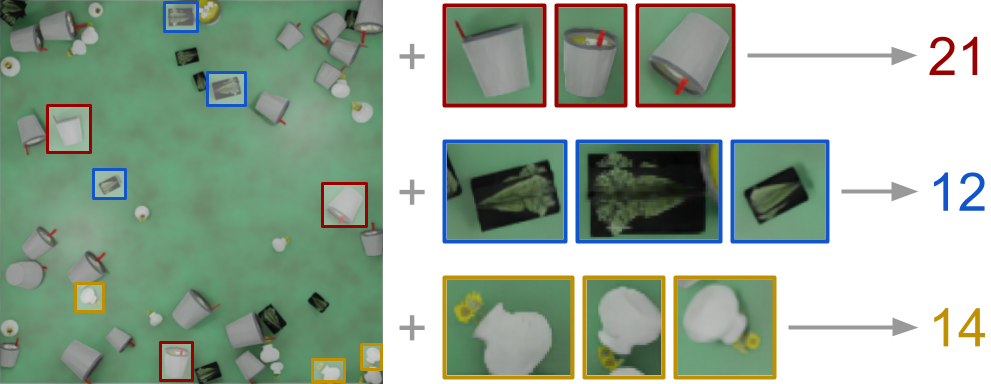
\includegraphics[width=0.85\linewidth]{../files/ABC123/images/teaser/ABC123 teaser-6.png}
        \caption{Exemplar-Based Counting
    }
    \end{subfigure}
        \begin{subfigure}{0.49\linewidth}
            \centering
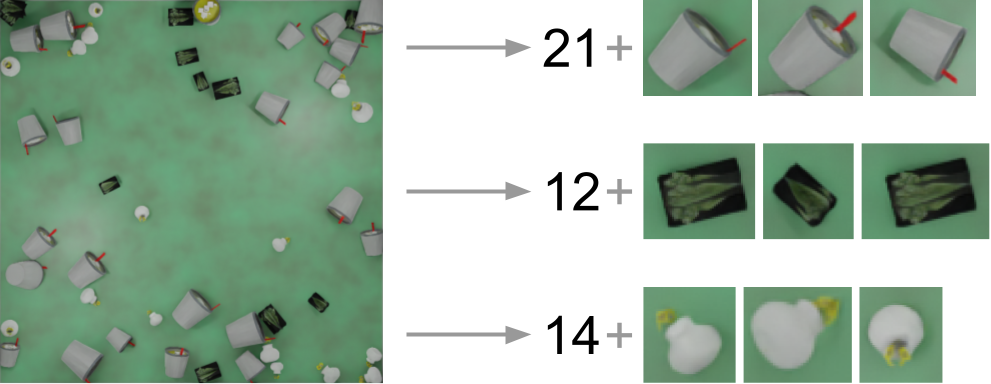
\includegraphics[width=0.85\linewidth]{../files/ABC123/images/teaser/ABC123 teaser-5.png}
        \caption{Our Exemplar-Free Counting
    }
    \end{subfigure}
    \caption{ABC123 counts objects of multiple unseen types. Our method not only does not need exemplars to define the type to count but also finds examples of each type it has counted.}
    \label{fig__ABC123__teaser}
\end{figure}

Our method, like many before \cite{ranjan2021Famnet,ranjan2022exemplar,liu2022countr,shi2022represent}, is based on density map regression.
For each image, there are $m$ classes present, each with an associated ground truth count $y$ and density map $d$. 
We regress $\hat{m}$ counts and density map predictions, $\hat{y}$ and $\hat{d}$ respectively. $\hat{m}$ acts as upper-bound of the number of counts ABC123 can regress.
\begin{equation}\label{eq__ABC123__CountAsDensityMapIntegral}
    \hat{y} = \sum_{h,w}{\hat{d}_{(h,w)}}
\end{equation} 
\myequations{Count as Density Map Integral}
where $\hat{d}_{(h,w)}$ denotes the density value for pixel (h, w).
We achieve this by using $\hat{m}$ convolutional up-sampling heads on top of a vision transformer backbone. 
We use a vision transformer backbone due to its globally receptive field and self-attention mechanism, which we showed is crucial to generating a complex understanding in counting settings in \Cref{sec__LTCA}.
Each head regresses a single pixel-wise density map prediction and count prediction from a patch-wise low-resolution high-dimensional feature space.
All of the count regression heads are identical and share their weights.

Similar to other contemporary methods \cite{ranjan2021Famnet, liu2022countr, yang2021cfoc, lin2021object}, we use the pixel-wise distance as our loss for the regression stage. Specifically, we use $||d - \hat{d}||_1$  where $d$ and $\hat{d}$ are the ground truth and predicted density maps.
This produced more accurate results than using the more common L$_2$ distance between the $d$ and $\hat{d}$; see the ablations tests in \Cref{sec__ABC123__ablation_losses} for the full comparison.

\begin{figure}
    \centering
    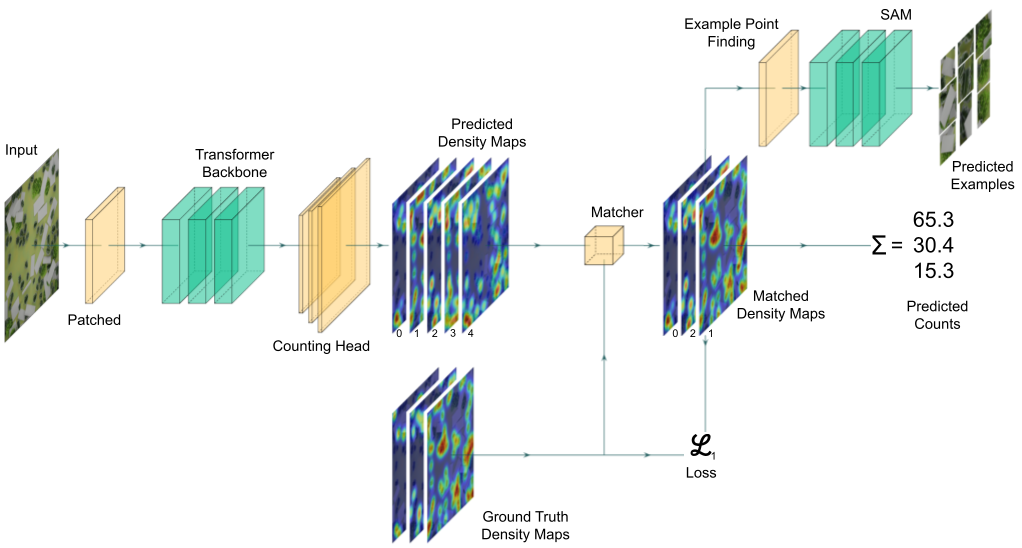
\includegraphics[width=\linewidth]{../files/ABC123/images/pipeline_drawing_updated_SAM.png}
        \caption{
    \textbf{The ABC123 pipeline.} 
    Our method learns to count objects of multiple novel classes without needing exemplar images. During training and quantitative evaluation, the matcher aligns the unguided predictions to the ground truth labels. The example prediction stage locates instances associated with each generated count.
    }
    \label{pipeline}
\end{figure}

\subsection{Matching}
In single-class or class-specific settings, there is a single prediction-label pair, one generated count and one ground truth class. 
In exemplar-based multi-class settings there is an introduced ambiguity as the exemplar images may not reflect the complete variation of the desired objects' appearances, \eg if the exemplars are of blue cars, should the network count only blue cars or all cars?
In multi-class exemplar-free settings, this ambiguity is increased significantly. There are multiple predictions as well as multiple labels, without a clearly defined pairing.
This resembles class-discovery \cite{troisemaine2023novel, Yang2010} and clustering \cite{Xie2016} problems, where the number and cardinality of new classes are not necessarily known. 

In keeping with these fields, we find correspondences between the set of $m$ known counts and the set of $\hat{m}$ predicted counts.
These correspondences are required to facilitate training and to evaluate the accuracy.
The binary correspondence matrix is defined as $\mathcal{X} = \{0,1\}^{m\times\hat{m}}$ where  $\mathcal{X}_{i,j}=1$ iff prediction $j$ is assigned to label $i$.
A problem instance is described by an $m\times\hat{m}$ cost matrix $\mathcal{C}$, where $\mathcal{C}_{i,j}$ is the cost of matching ground truth label $i$ and prediction $j$. 
The goal is to find the complete assignment of predictions to labels with minimal cost.
Formally, the optimal assignment has a cost
\begin{equation}\label{eq__ABC123__Bipartite_matching}  \min_{\mathcal{X}}\sum_{i=0}^{m}\sum_{j=0}^{\hat{m}}\mathcal{C}_{i,j} \cdot \mathcal{X}_{i,j}
\end{equation}
\myequations{Bipartite Matching Assignment}
Specifically, our cost function is defined as the pixel-wise distance of the normalised ground truth density map $d_i$ and the predicted density map $\hat{d}_j$. 
\begin{equation} \label{eq__ABC123__MAPE_cost}
\mathcal{C}_{i,j} = \left|\left| \frac{d_i}{||d_i||_2} -  \frac{\hat{d}_j}{||\hat{d}_j||_2} \right|\right|_2 
\end{equation}
\myequations{Pixel-Wise Matching Cost}
The normalisation ensures the matching is done on the locality of the counted objects rather than the magnitude of the prediction itself. We found empirically that this stricter constraint improves the convergence speed of the network to generate density maps that localise the instances.
We use the Hungarian algorithm \cite{Kuhn1955}, specifically the Jonker-Volgenant algorithm outlined in \citet{Crouse2016hungarianmatching}, to solve for $\mathcal{X}$ robustly.

The supervision loss for each image is the sum of the L$_1$ difference of  all of the ground truth density maps and their matched predictions as:
\begin{equation} \label{eq__ABC123__total_loss}
\mathcal{L} = \sum_{i,j}^{m,\hat{m}}||d_i - \hat{d}_j||_1 \cdot \mathcal{X}_{i,j}
\end{equation}
\myequations{L$_1$ Density Map Loss}
It should be noted that every label has an associated prediction, but the inverse is not the case, as generally $\hat{m} > m$.
This means we do not impose a loss on the unmatched density maps.
This allows the network to generate more nuanced count definitions as it does not punish valid-but-unknown counts which are likely present in any counting setting.

As is usual \cite{troisemaine2023novel, Yang2010, DMShobley,Xie2016}, we use the same matching procedure to quantitatively evaluate our performance at inference-time. 
It should be noted that as this matching stage uses the ground-truth density maps, it could be used to significantly benefit a method's quantitative results without improving its deployment capabilities.
Specifically, a method could in theory predict all possible density maps and use the matching stage to pick the correct one.

As MCAC has a maximum of 4 classes present in an image, we limit our method to generating 5 density maps to minimise this behaviour.
The effect of this is explored in the ablation tests in \Cref{sec__ABC123__ablation_mhat}.
We also normalise the density maps between 0 and 1 to ensure we are only matching to the locations of objects rather than the counts themselves.
We explore the impact of this normalisation in more detail in the ablation tests in \Cref{sec__ABC123__ablation_matchers}.

\subsection{Example Discovery}
While exemplar-free counting saves a user time, as no manual intervention is required, it does require the user to interpret the results. 
A set of scalar count values can be unclear as it is not always obvious which count corresponds to which type of object in the input image. 
Density maps can also often be difficult to interpret, especially in high-density situations; see \Cref{fig__ABC123__MCAC_vis} for examples of difficult-to-interpret counts and density maps.

To aid the user in understanding to which class a generated count corresponds, we propose flipping the usual exemplar-based paradigm.
Instead of using exemplar images to define the type to count, we find examples of the type counted. 
We achieve this by finding points that are likely to belong to instances of the counted class from the predicted density map and using them as seed inputs for a pre-trained class-agnostic segmentation method \cite{kirillov2023segany}. 
For class $i$, we find a set of representative points, $\mathcal{P}_i = \{p_{i,0}, p_{i, 1},...\ , p_{i, n}\}$, by locating pixel locations that have a high activation in the density map for class $i$, $\hat{d}_i$, and a low activation in the density maps for the other predicted classes, $\hat{d}_j$.
Formally:
\begin{equation}
    p_{i,0} = \argmax_{h,w}\left(\hat{d}_{i, (h,w)} - \max_{j\neq i}\left(\hat{d}_{j, (h,w)}\right)\right)
\end{equation}
\myequations{Locating Initialisation Points for Example-Finding}
\noindent where $\hat{d}_{i, (h,w)}$ is the value of pixel $(h, w)$ of the regressed density map for class $i$.

To find a diverse set of initialisation points for multiple instance examples, we exclude an area around $p_{i,0}$ when searching for $p_{i, 1}$. 
To capture the range of variation of the counted instances, we select the three points from $\mathcal{P}_i$ which have the largest latent feature distance in the final layer of the transformer backbone to use as our 3 initialisation points.
We use these points as seed inputs for a pre-trained segmentation method, SAM \cite{kirillov2023segany}.

The end user is presented with cropped areas of the query image centred on these segmentations. See \Cref{fig__ABC123__example_discovery} for visual presentations of cases with counts and found examples.
We use this approach because SAM is often not accurate enough to segment a singular whole object given only a singular point, as is shown in \Cref{fig__ABC123_sam_failures}.
However, the expanded bounding boxes provide more context, allowing an end user to infer the object counted.

\begin{figure}
    \centering    
    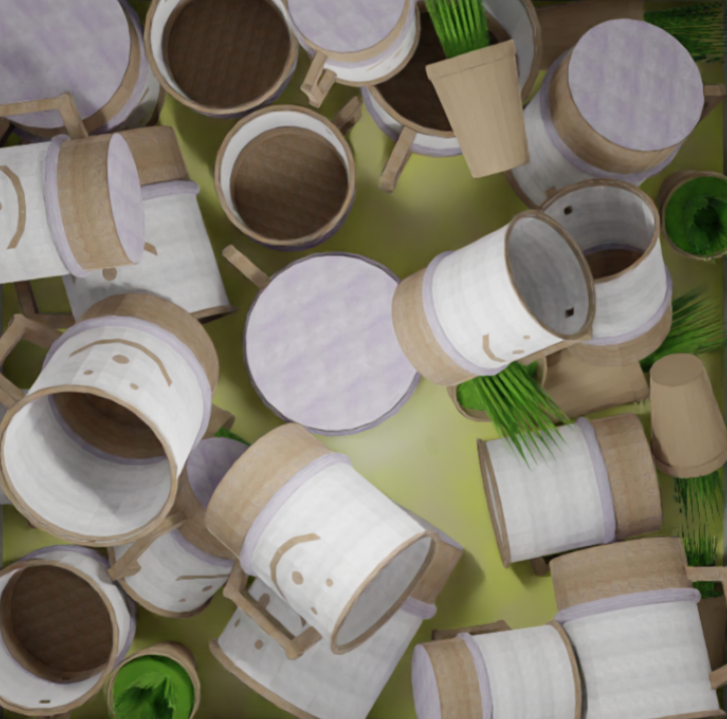
\includegraphics[width=0.22\linewidth]{../files/ABC123/images/sam_failures/144576663096439.png}    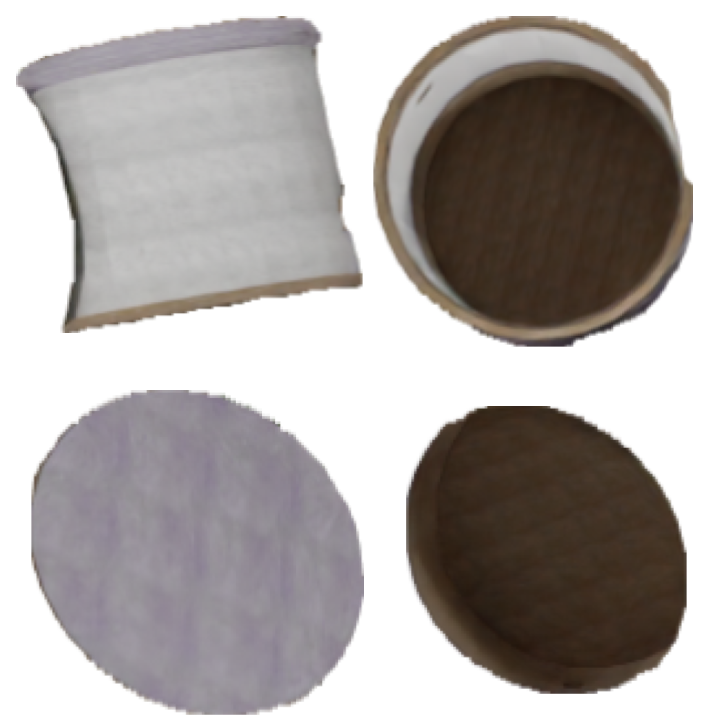
\includegraphics[width=0.22\linewidth]{../files/ABC123/images/sam_failures/144576663096439_segs.png}\hfill  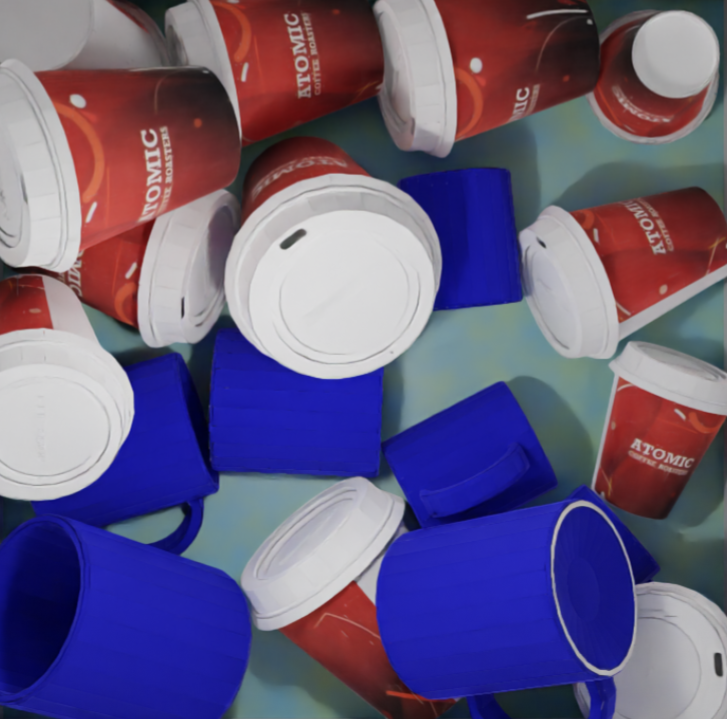
\includegraphics[width=0.22\linewidth]{../files/ABC123/images/sam_failures/2586631032094013.png}    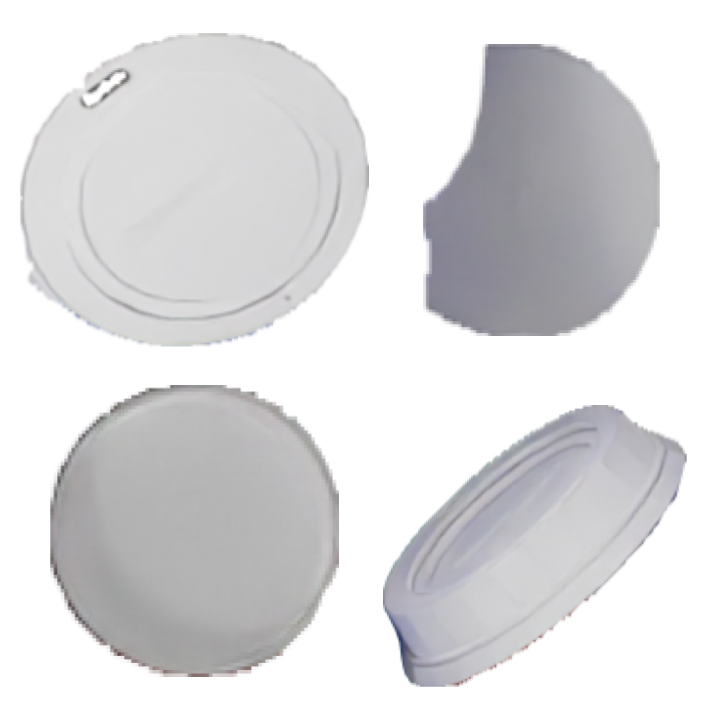
\includegraphics[width=0.22\linewidth]{../files/ABC123/images/sam_failures/2586631032094013_segs.png}\\
    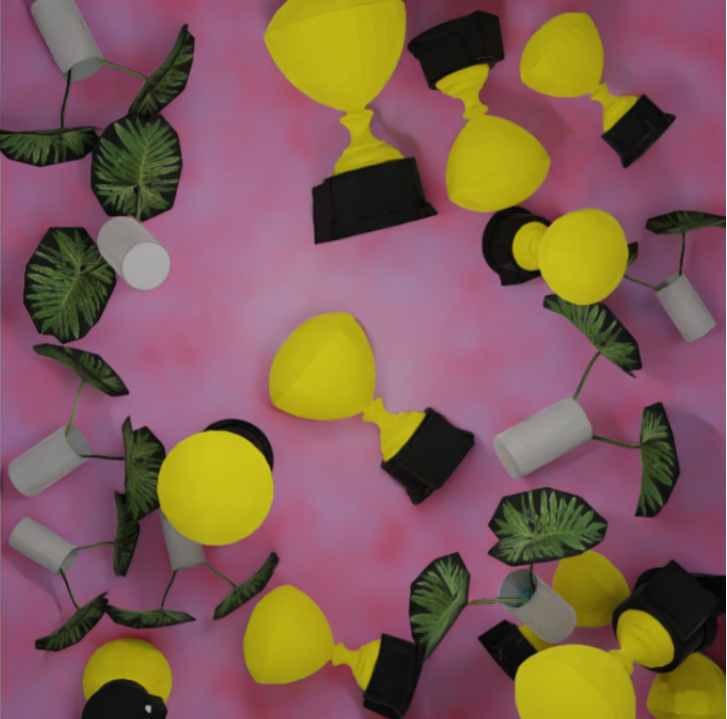
\includegraphics[width=0.22\linewidth]{../files/ABC123/images/sam_failures/918828767031931.png}    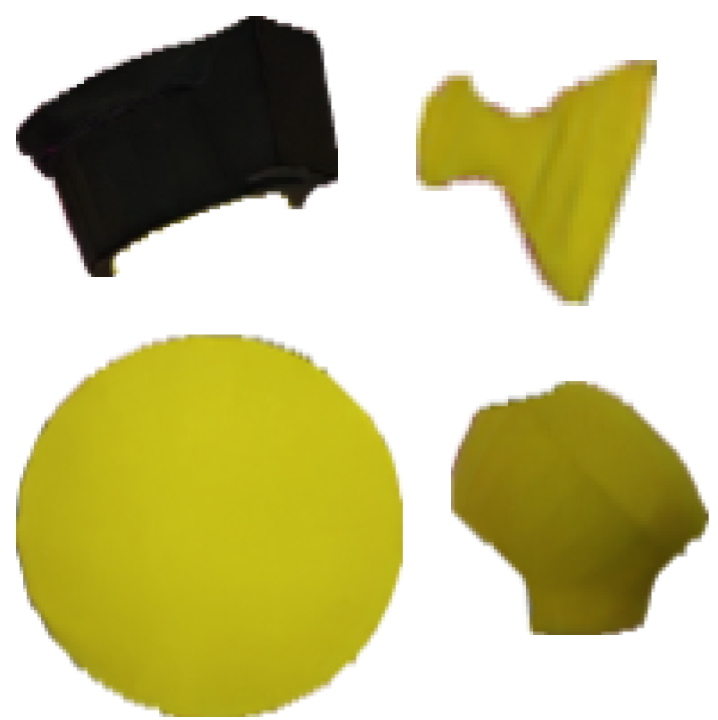
\includegraphics[width=0.22\linewidth]{../files/ABC123/images/sam_failures/918828767031931_segs.png}\hfill
    
\includegraphics[width=0.22\linewidth]{../files/ABC123/images/sam_failures/2698668580807301.png}    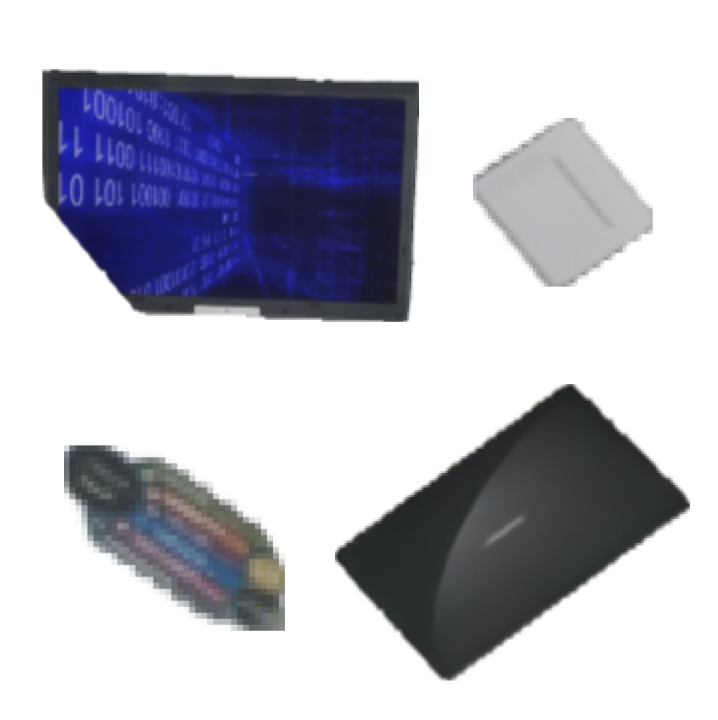
\includegraphics[width=0.22\linewidth]{../files/ABC123/images/sam_failures/2698668580807301_segs.png}
    \caption{Examples from a naive example finding stage using peak finding and a pre-trained segmentation method \cite{kirillov2023segany}. Often, the found segmentations are not a representation of the whole counted object and so are not informative for the user.}
    \label{fig__ABC123_sam_failures}
\end{figure}

\begin{figure}
    \centering    

    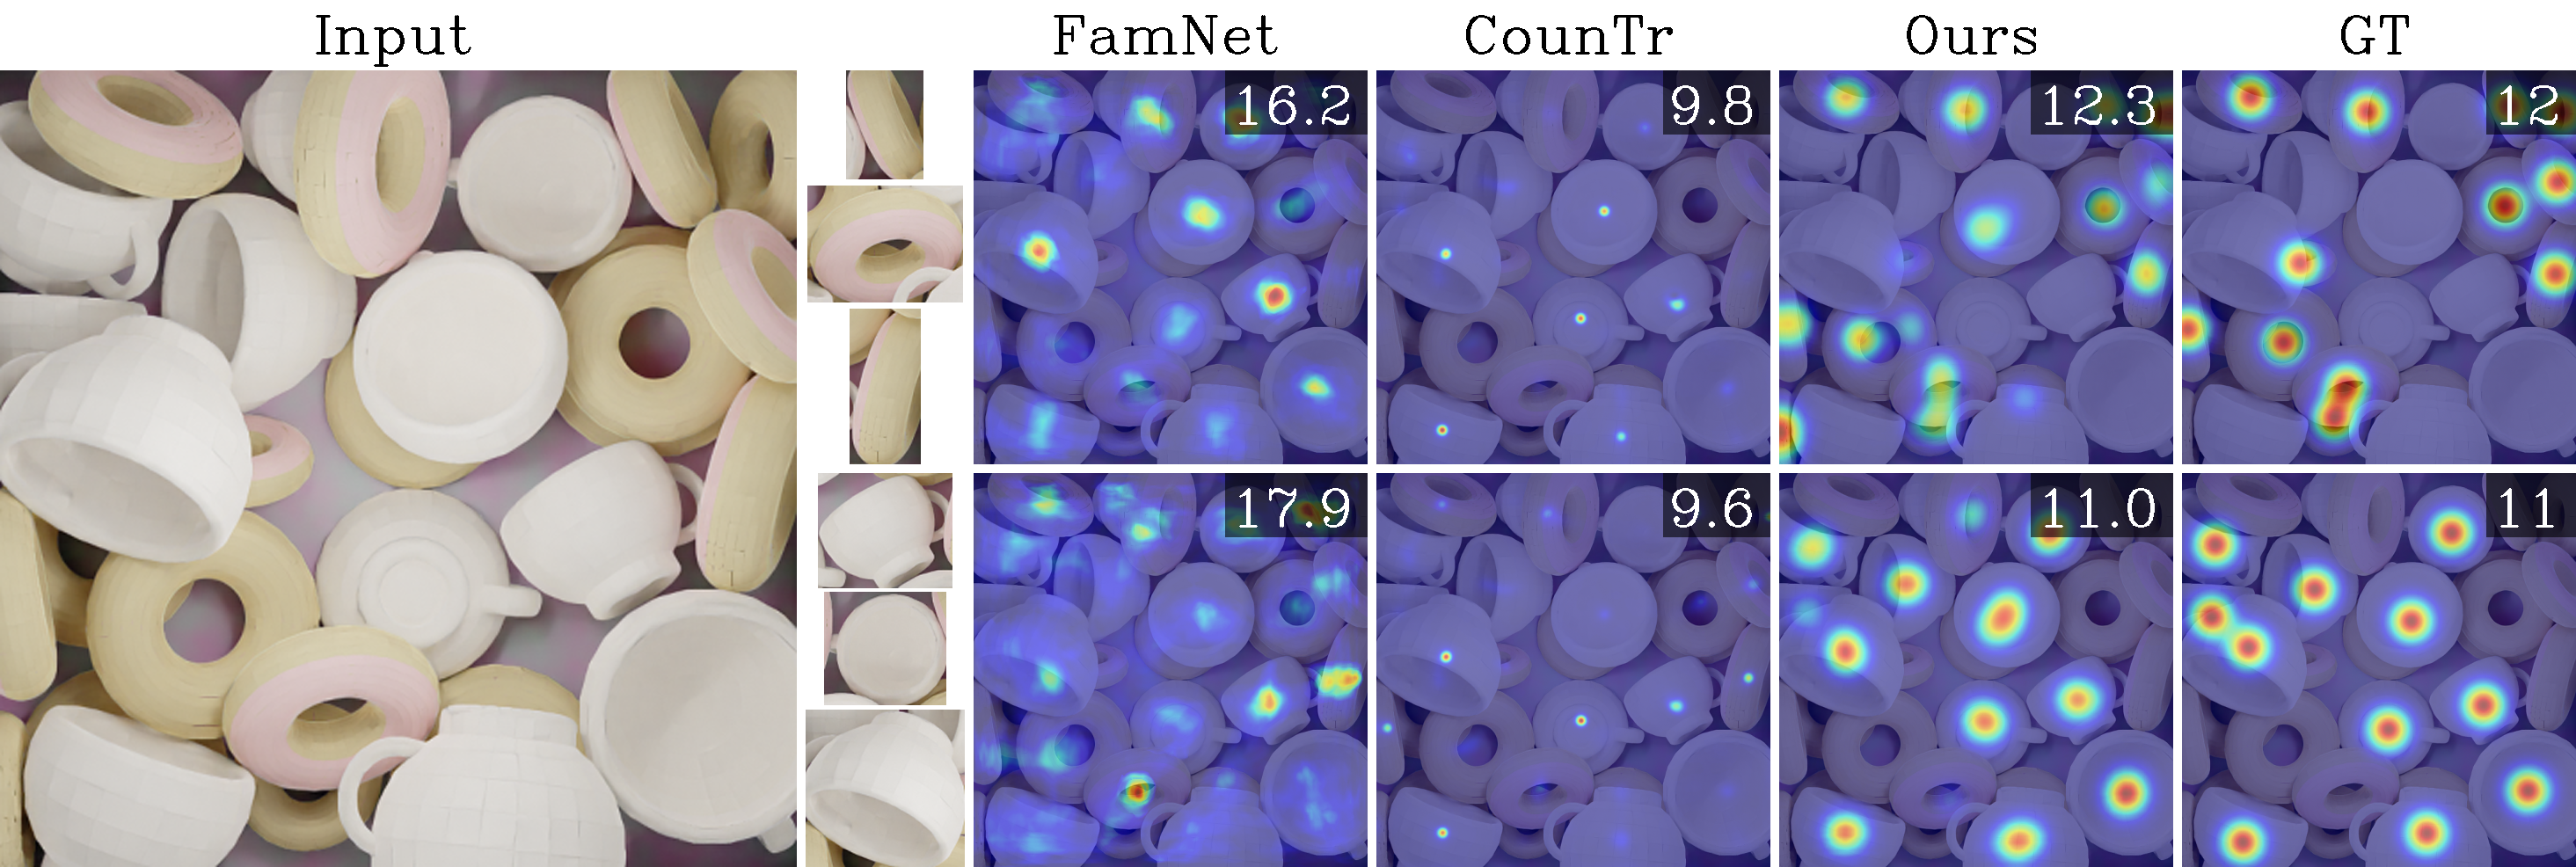
\includegraphics[width=\linewidth]{../files/ABC123/images/blender_comparison/1666939059059935.png}\\
    \vspace{1mm}
    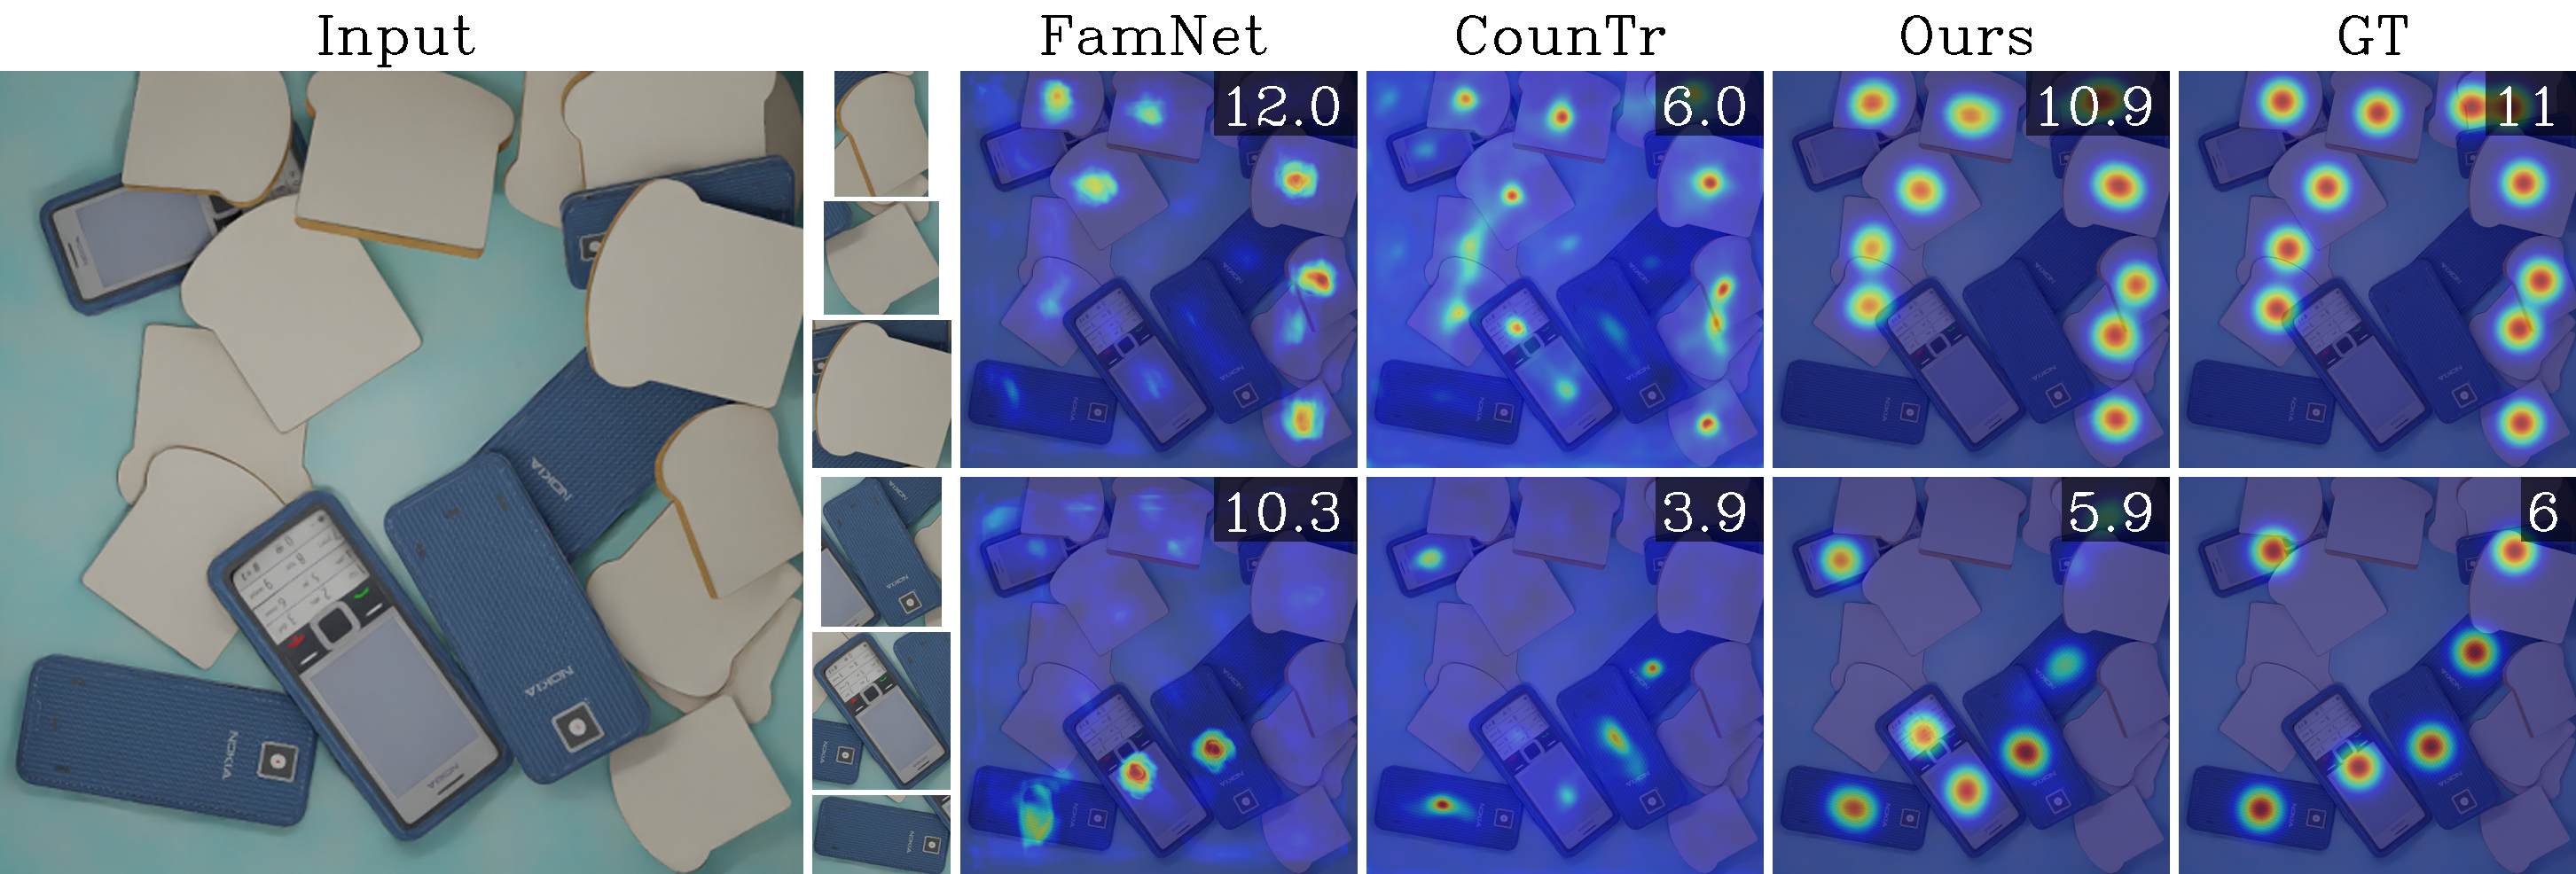
\includegraphics[width=\linewidth]{../files/ABC123/images/blender_comparison/2200837159622185.png}\\
    \vspace{1mm}
    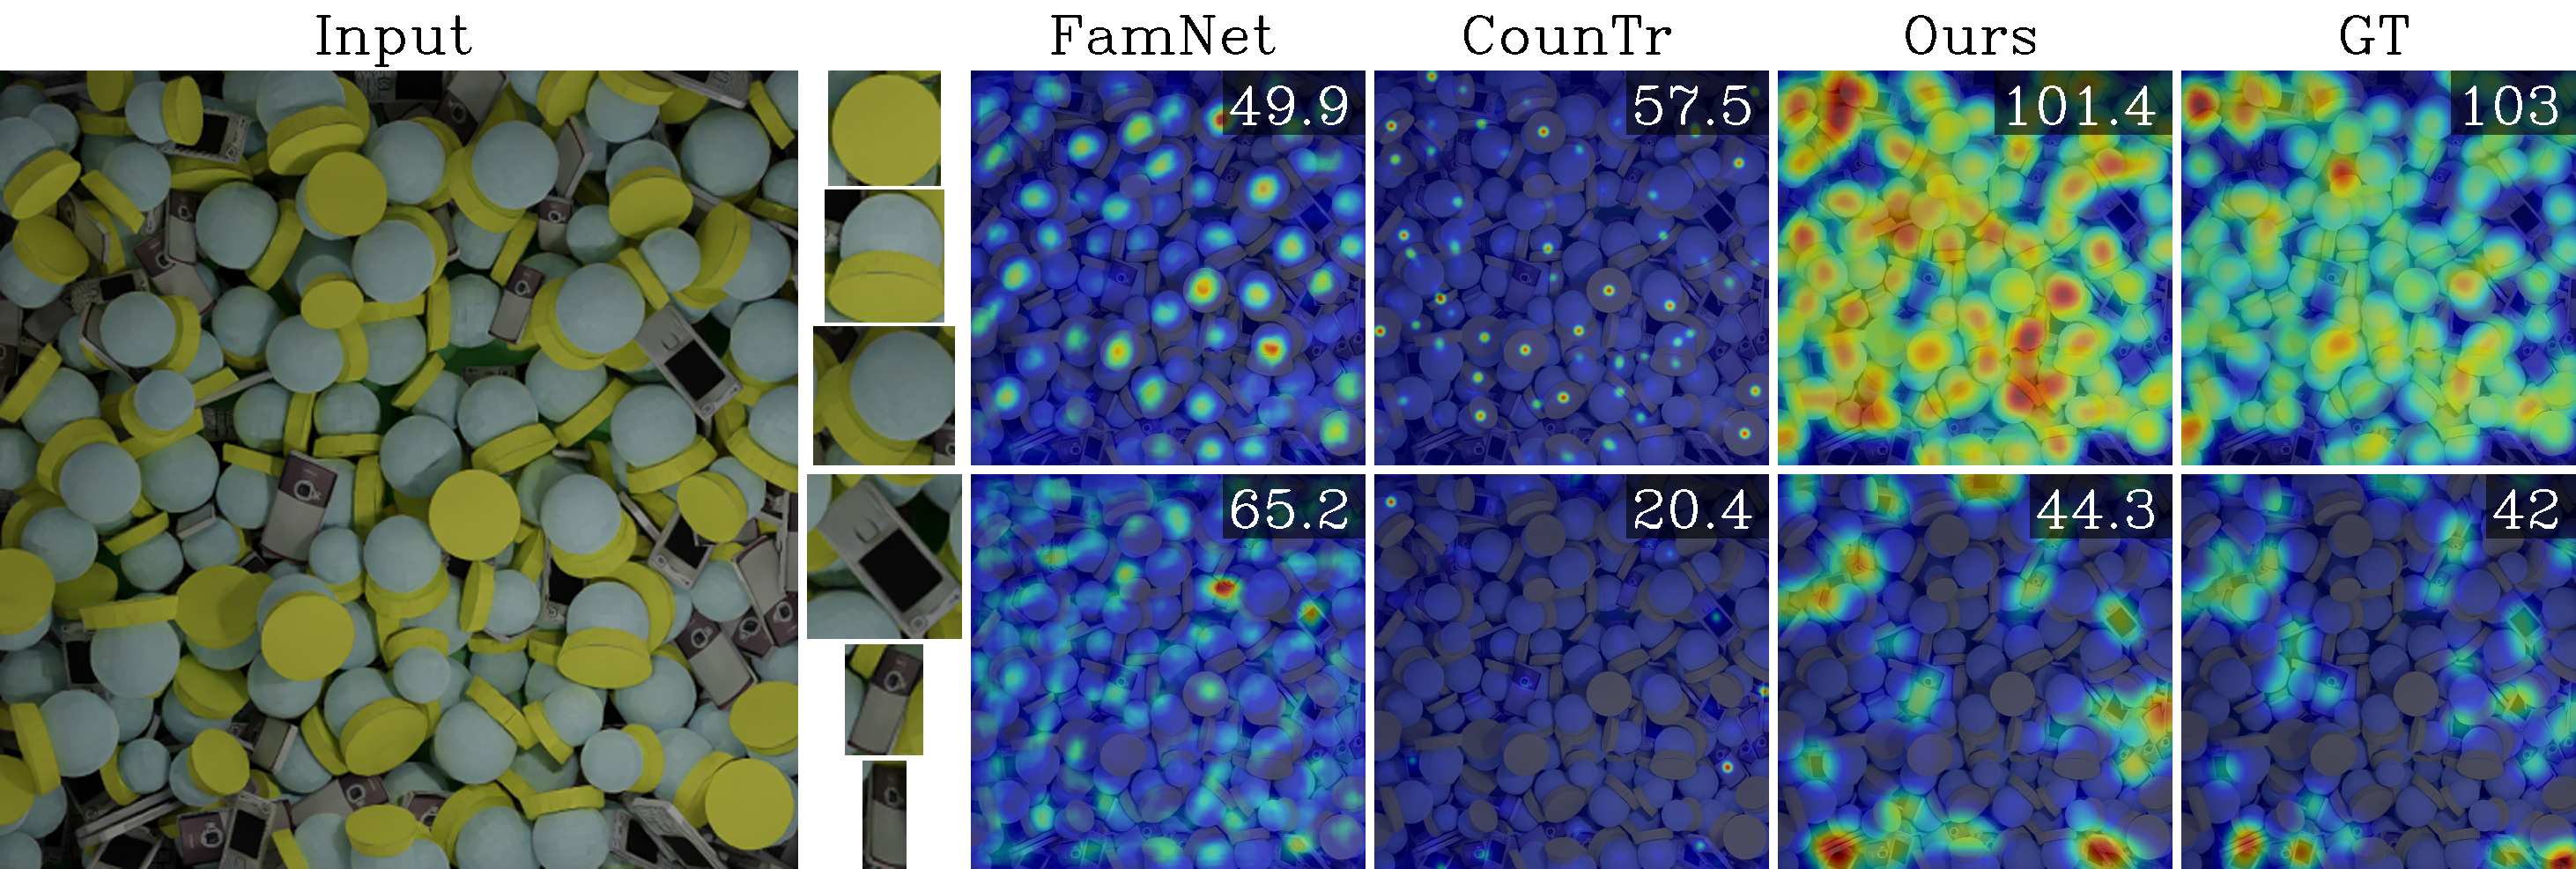
\includegraphics[width=\linewidth]{../files/ABC123/images/blender_comparison/2534708946430548.png}\\
    \vspace{1mm}
    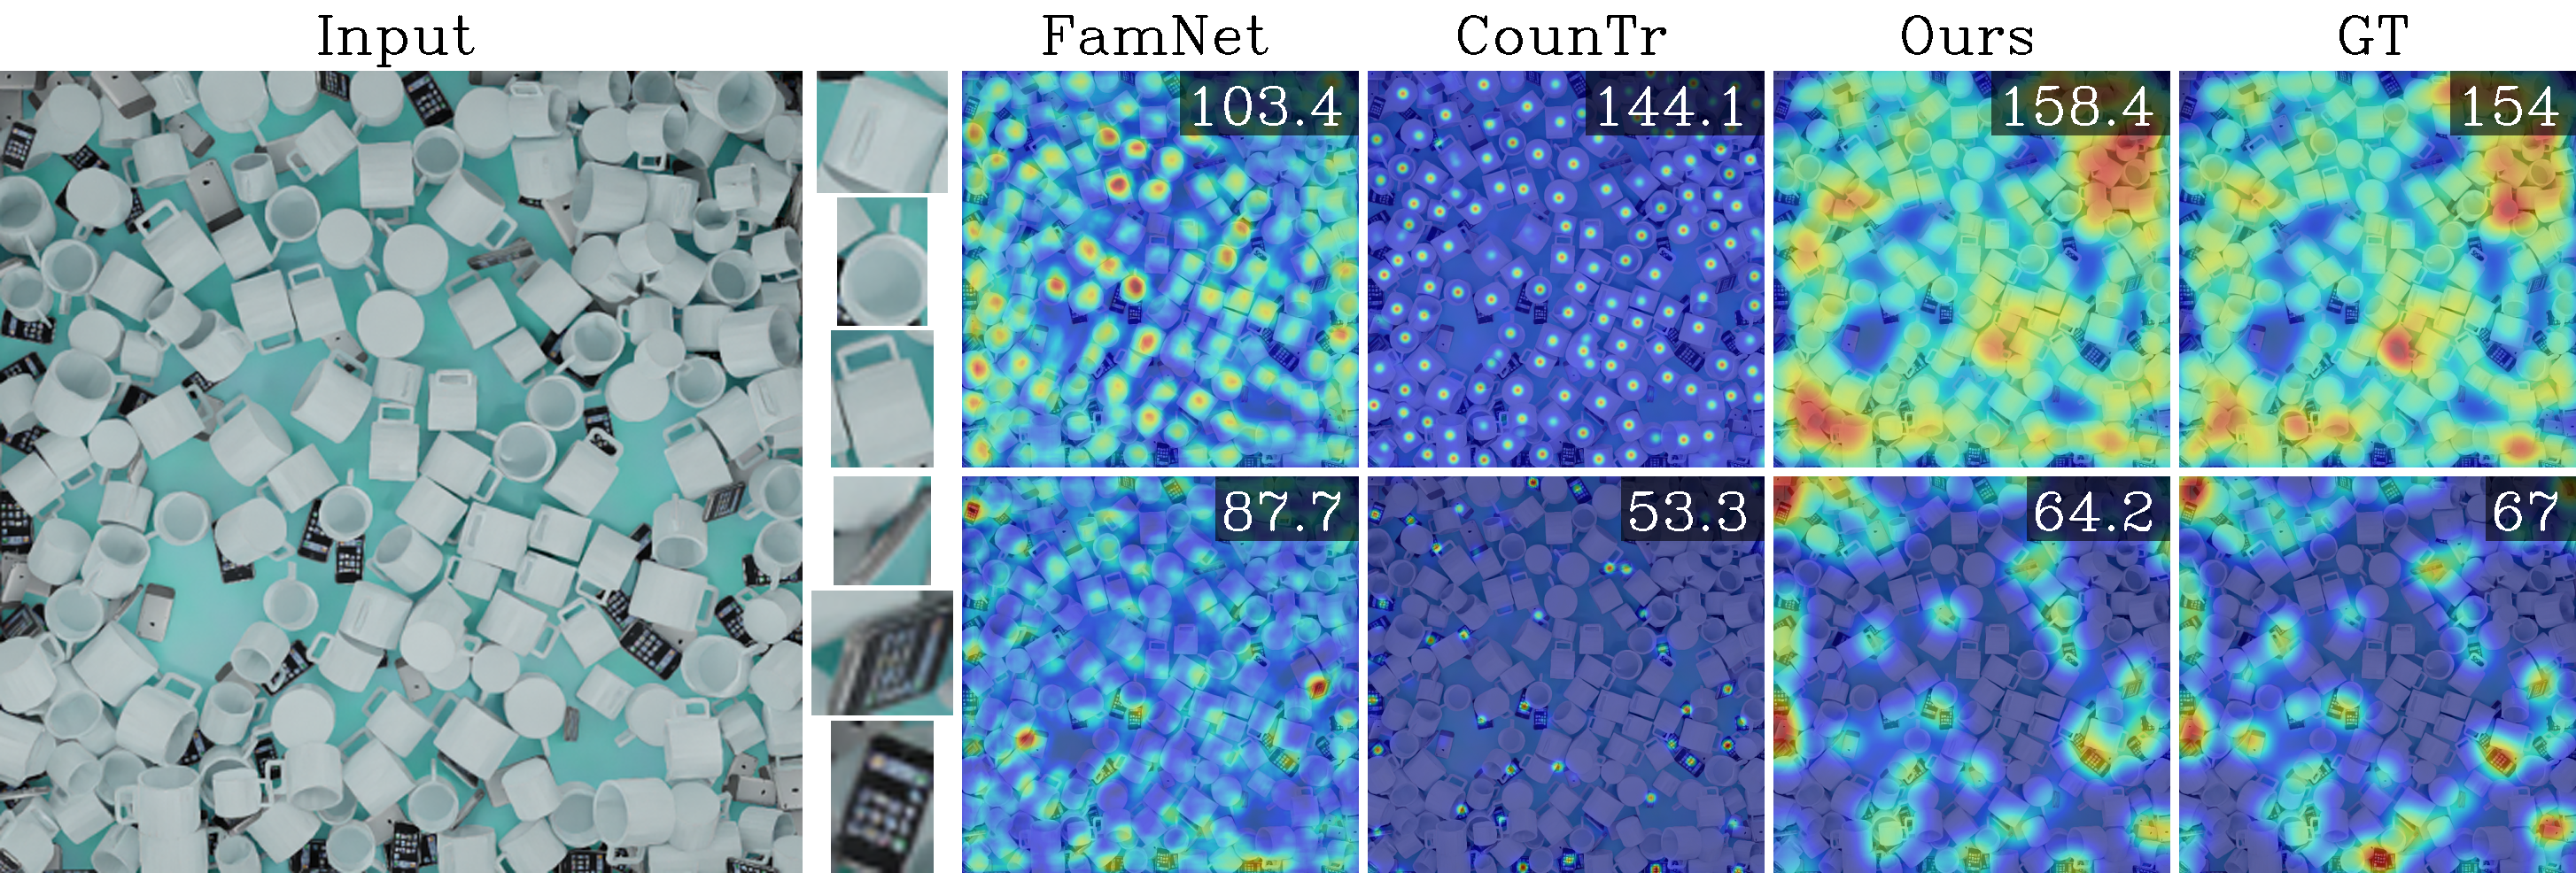
\includegraphics[width=\linewidth]{../files/ABC123/images/blender_comparison/2671656807687632.png}
        \caption{
    \textbf{Comparison to other methods on MCAC.} 
    ABC123 produces more accurate results than the exemplar-based methods without using exemplar images.
    The ground truth (GT) and  predicted counts are shown in the top right corner of their respective density maps.
    }
    \label{fig__ABC123__MCAC_vis}
\end{figure}

\begin{figure}
    \centering    
    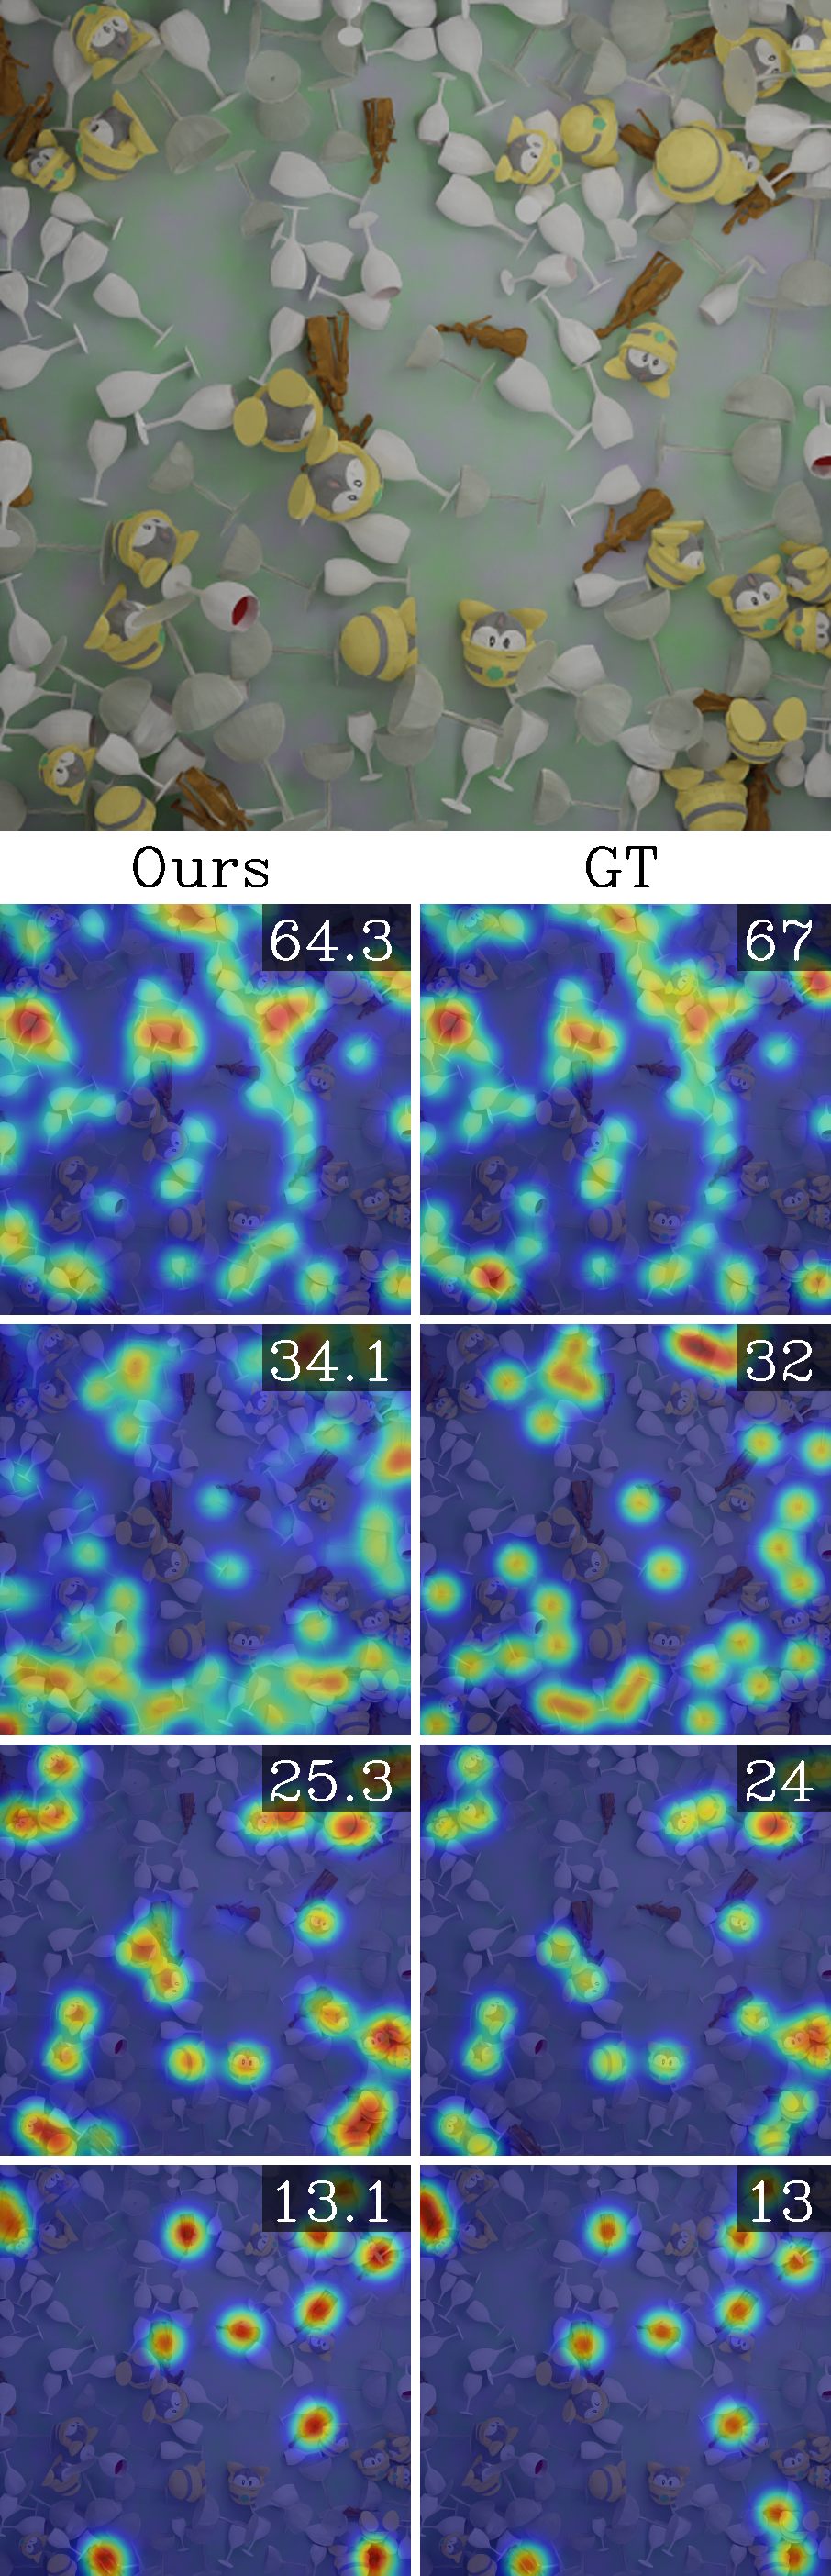
\includegraphics[width=0.4\linewidth]{../files/ABC123/images/4s/5224022009776293.png}
    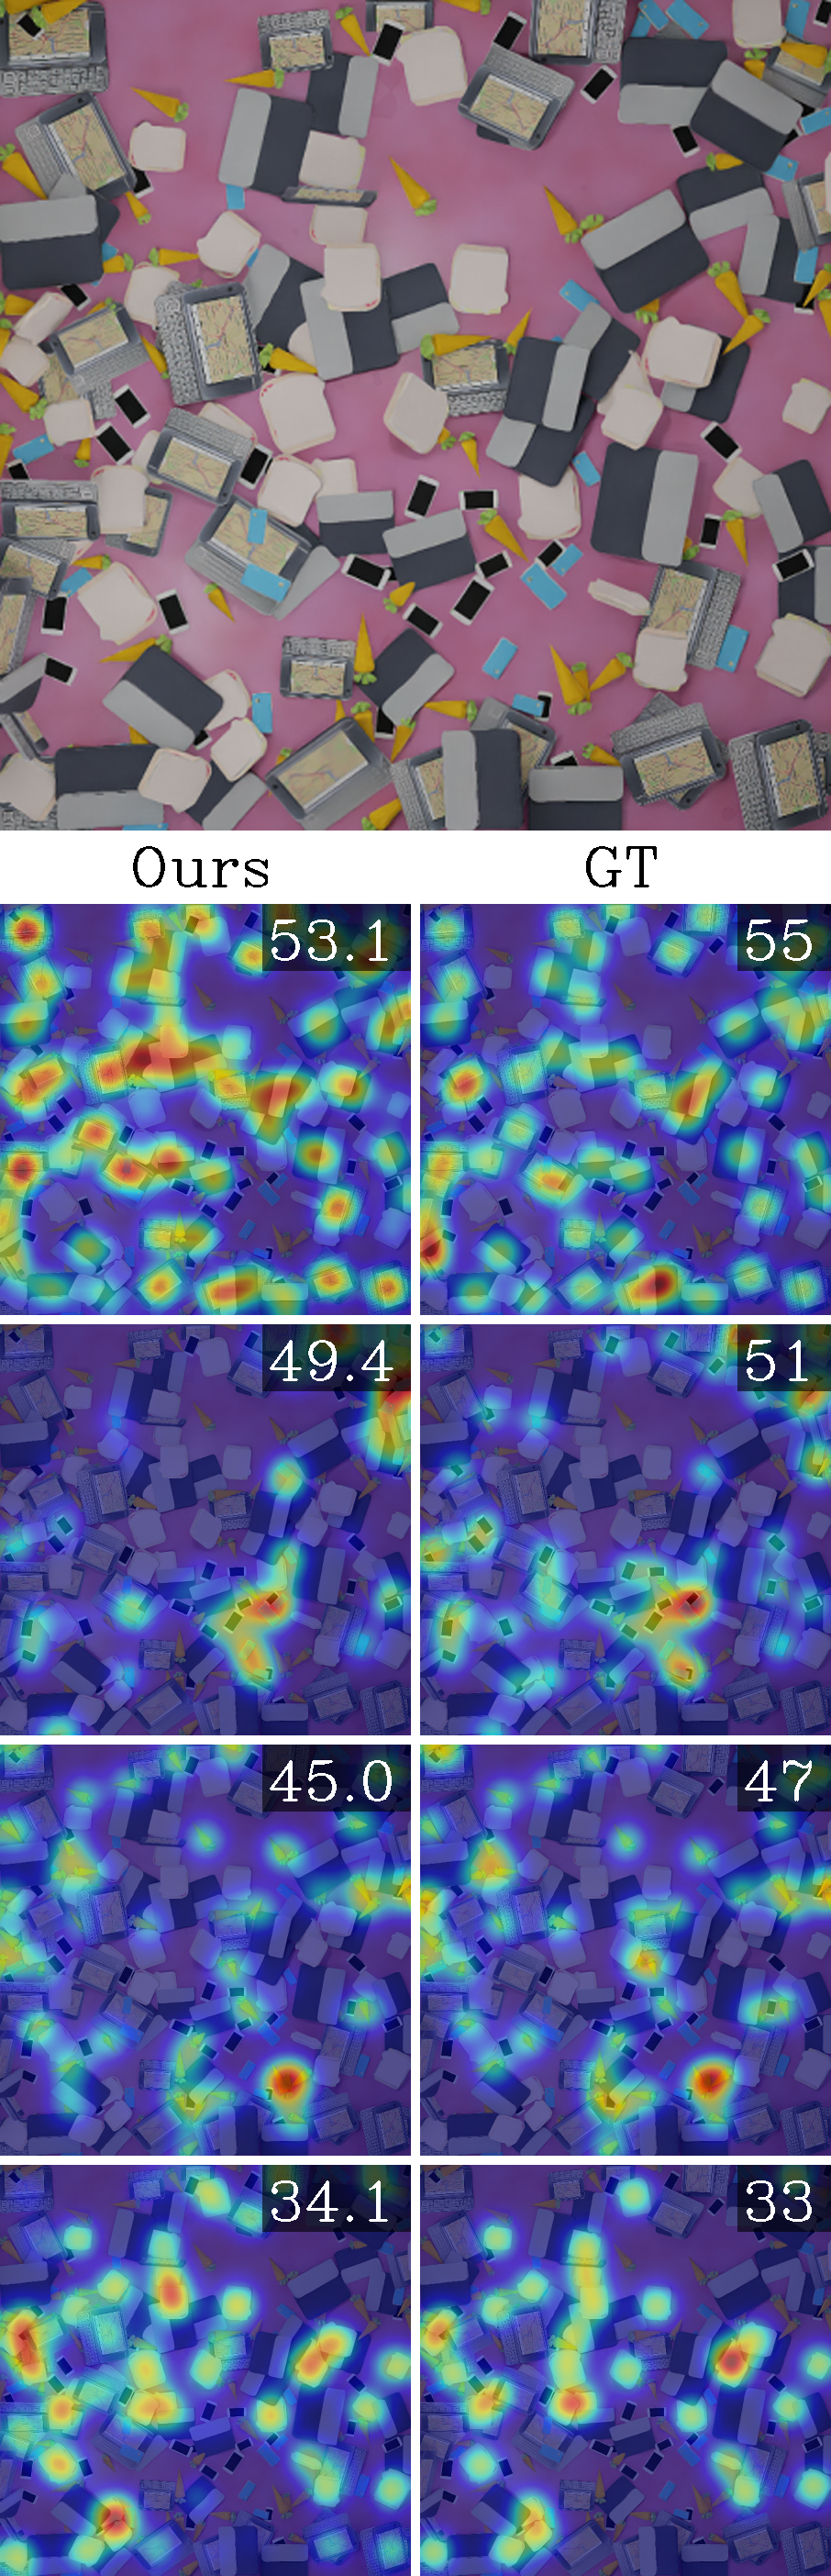
\includegraphics[width=0.4\linewidth]{../files/ABC123/images/4s/9075293767875800.png}
        \caption{
    \textbf{Results of our method on images with 4 classes.} 
    ABC123 can generate accurate counts and meaningful density maps from images with four novel classes. MCAC has between one and four classes of objects per image.
    }
    \label{fig__ABC123__MCAC_vis_4_classes}
\end{figure}




\begin{figure}
    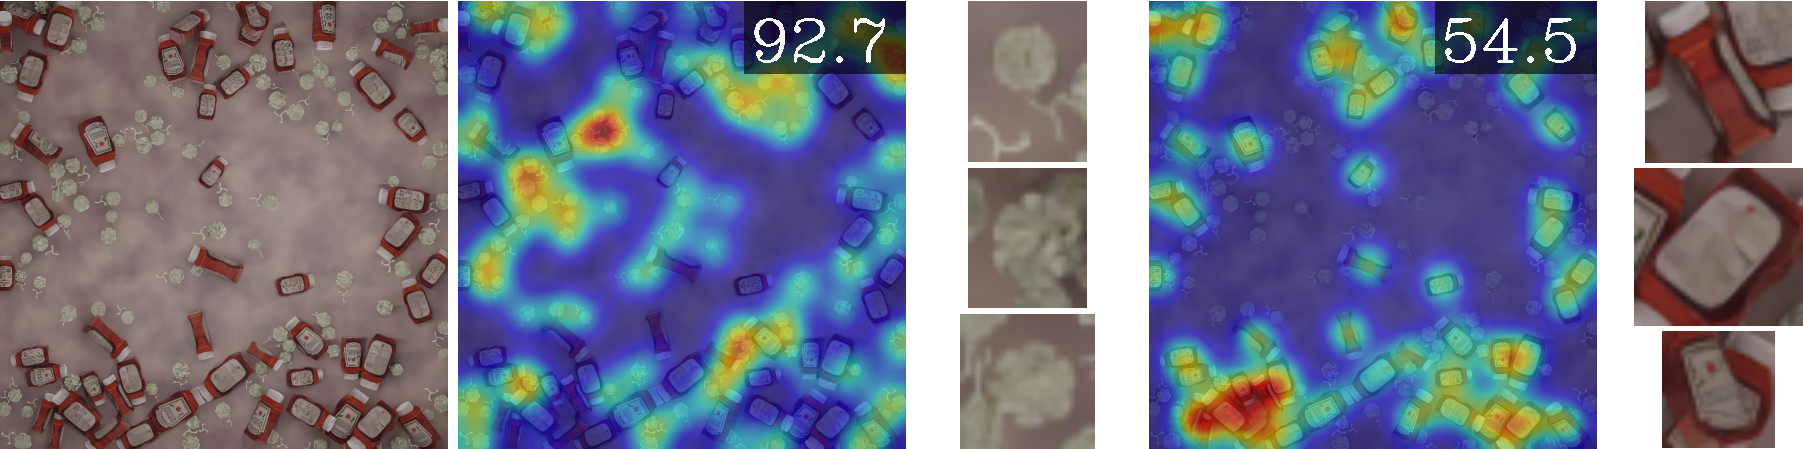
\includegraphics[width=0.99\linewidth]{../files/ABC123/images/bounding_box_finding/SAM_found_bboxes_1991666512496129.png}
\vspace{0.5mm}\\
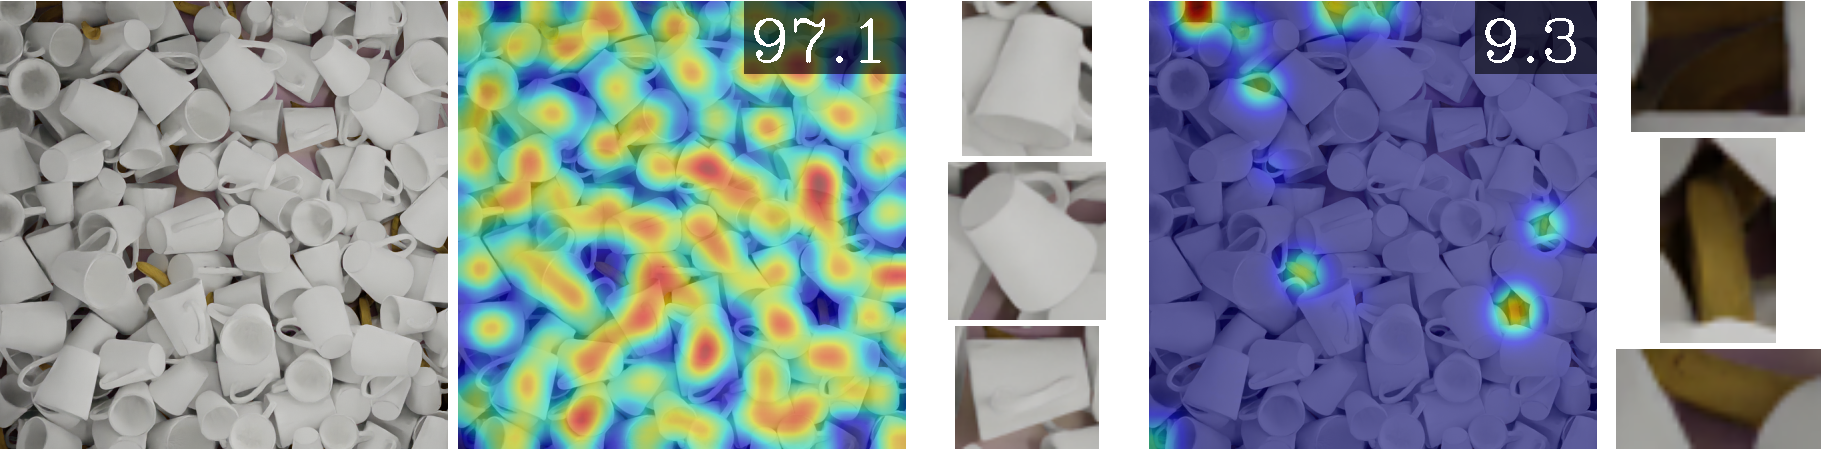
\includegraphics[width=0.99\linewidth]{../files/ABC123/images/bounding_box_finding/SAM_found_bboxes_2751222122226916.png}
\vspace{0.5mm}\\
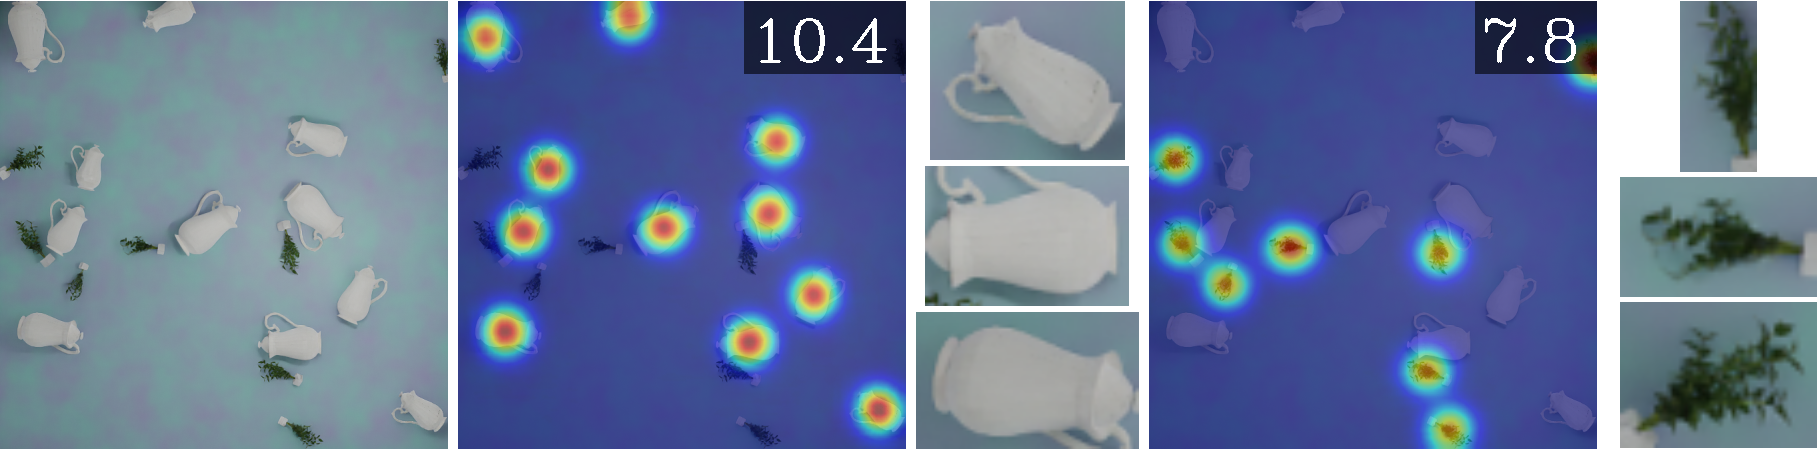
\includegraphics[width=0.99\linewidth]{../files/ABC123/images/bounding_box_finding/SAM_found_bboxes_2743168248170490.png}
\vspace{0.5mm}\\
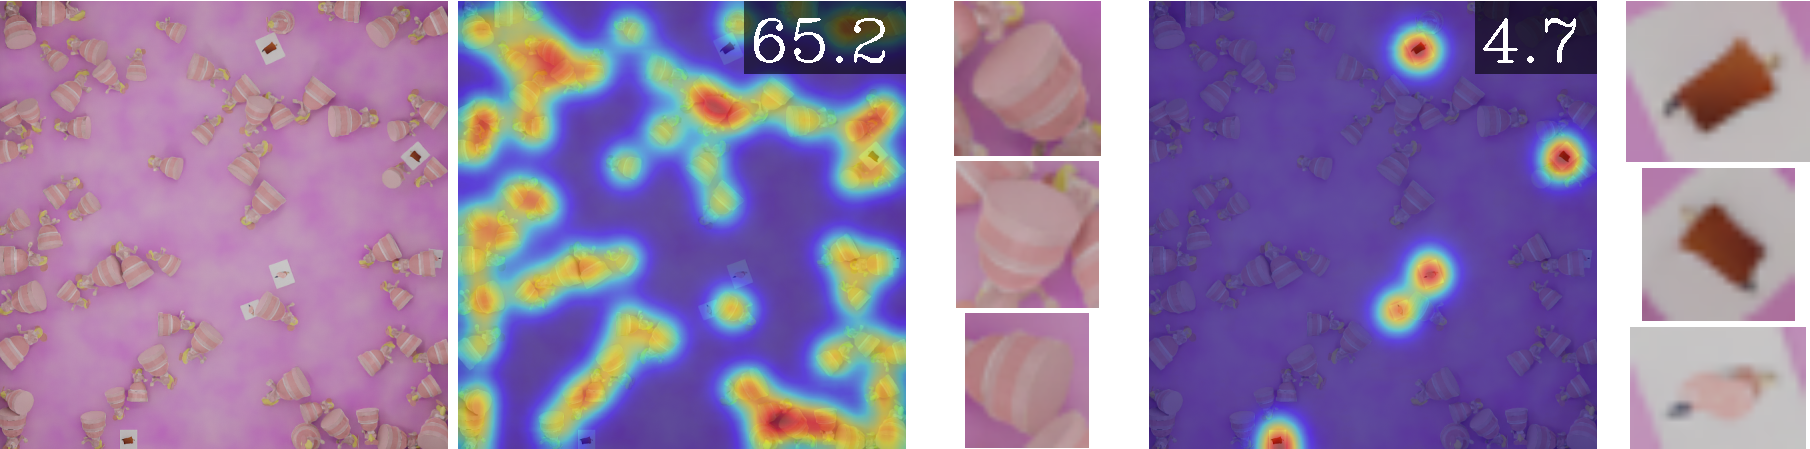
\includegraphics[width=0.99\linewidth]{../files/ABC123/images/bounding_box_finding/SAM_found_bboxes_2854740766783037.png}
\vspace{0.5mm}\\
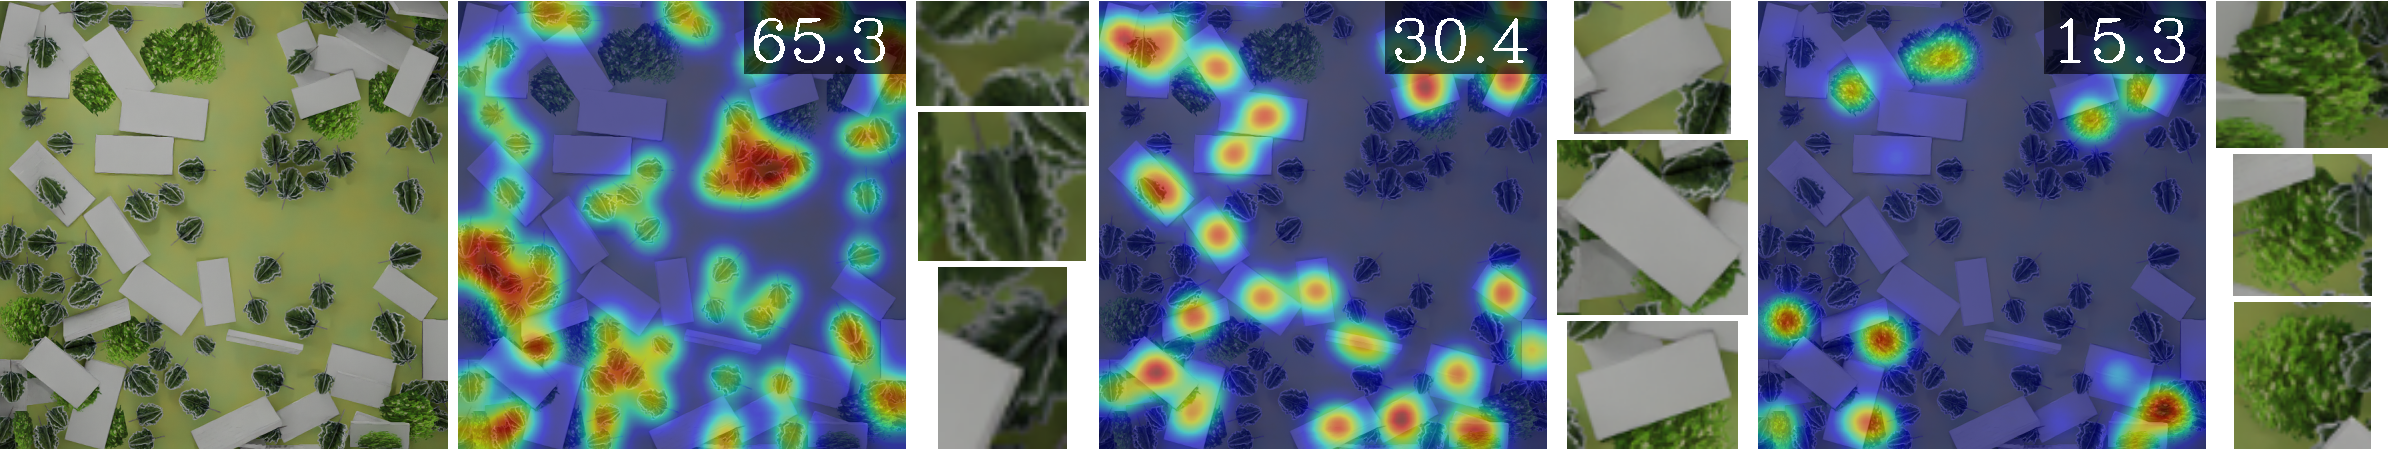
\includegraphics[width=0.99\linewidth]{../files/ABC123/images/bounding_box_finding/only_gen_bboxes_742340842329572_notbad.png}
\vspace{0.5mm}\\
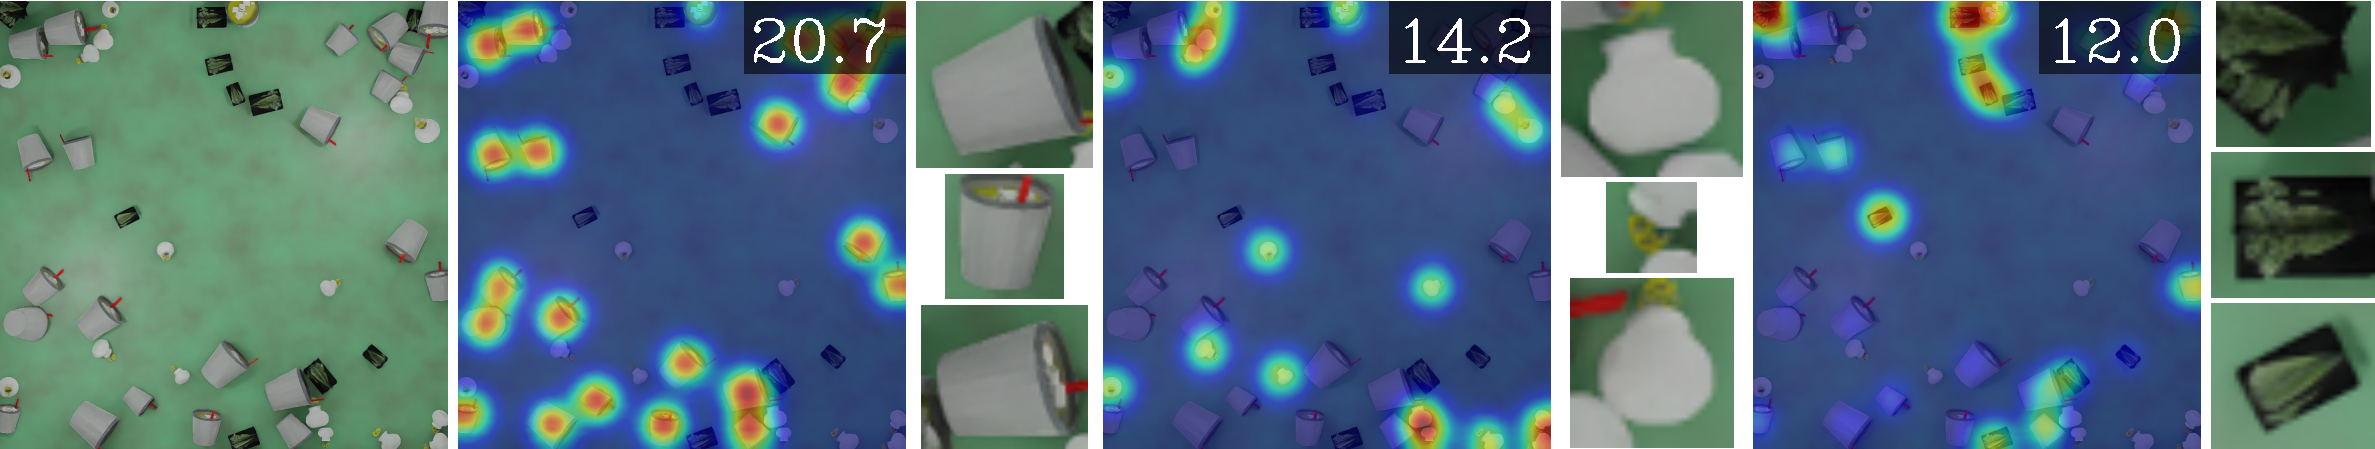
\includegraphics[width=0.99\linewidth]{../files/ABC123/images/bounding_box_finding/only_gen_bboxes_2041963832336316_notbad.png}%
    \caption{
    \textbf{Example Finding.} Using our density map predictions, we generate example bounding boxes to aid a user in understanding what has been counted.
    }
    \label{fig__ABC123__example_discovery}
\end{figure}

\subsection{Implementation}
We use the ViT-Small \cite{dosovitskiy2020vit} architecture for our backbone due to its lightweight nature and for a fair comparison to methods that use the Resnet-50 backbone, such as FamNet\cite{ranjan2021Famnet}  and BMNet \cite{shi2022represent}.
ViT-S has a similar number of parameters, throughput, and supervised ImageNet performance as ResNet-50 \cite{touvron2021training}.
Due to this lightweight backbone, ABC123 is trainable in less than eight hours using two Nvidia 1080Ti GPUs. 
It takes less than two hours to train just the head with a frozen pre-trained backbone (ABC123\textsmaller[2]{\SnowflakeChevron}).

Since vision transformers typically demand substantial training data, we initialised our transformer backbone with weights sourced from \citet{caron2021DINO} in the same way as in \Cref{sec__LTCA}.
This self-supervised pre-training process endows the network with an understanding of meaningful image features before exposure to our dataset and without supervision. This approach reduces the risk of overfitting when the model is then trained on our dataset.

Our counting heads increase the patch-wise resolution of the trained counting features from $k \times (28\times28)$ to a pixel-wise density map prediction of $\hat{m} \times (224\times224)$,
where $k$ is the dimensionality of the transformer features and $\hat{m}$ is the maximum number of predicted counts. For ABC123, $k = 384$.
Each counting head is comprised of  a linear projection from $384\times(28\times28)$ to a $(\hat{m}\times16)\times(28\times28)$ feature space.
This is then split into $\hat{m}$ separate $16\times28\times28$ feature maps, each of which is then upsampled to regress $\hat{m}$ pixel-wise density maps. 
The upsampling is comprised of 3 Conv-ReLU-Upsample blocks followed by a convolutional layer. Each upsampling operation bilinearly interpolates features increasing the resolution by 2$\times$. Each convolutional layer decreases the feature dimensionality by $\frac{1}{2}$. We use a $7\times7$ convolutional kernel for each stage in order to increase the receptive field of this upsampling. 

As the largest number of classes in a single image in MCAC is four ($m\leq4$), we set $\hat{m} = 5$. This is the minimum number that ensures that the method has the capacity to generate a count for every defined class in a given image as well as at least one valid-but-unknown count, the value of which is discussed in more detail in \Cref{sec__ABC123__ablation_vbu}. The effect of varying $\hat{m}$ on both quantitative results and deployment time utility is further discussed in the ablation tests in  \Cref{sec__ABC123__ablation_mhat}.

Our choice of the ViT-Small backbone limits the resolution of our input image to (224$\times$224) as opposed to the $\geq$(384$\times$384) resolution used by contemporary methods with ResNet-50 or larger ViT backbones. However, it increases the ability to train the method on a broader range of hardware and allows for a fairer comparison to other contemporary methods.
For the example discovery stage, we use a frozen pre-trained ViT-B SAM model backbone \cite{kirillov2023segany} to generate the original segmentations. 


\section{Results}\label{sec__ABC123__results}
In this section, we outline how we will fairly compare our method to other recent counting methods before demonstrating the superiority of ABC123 to those methods.

\subsection{Benchmarking Methods}
We evaluate our method against two trivial baseline methods which predict the training-set mean or median count for all inference images, as in \Cref{sec__LTCA__benchmarking_methods}. As there are no previous multi-class exemplar-free class-agnostic counting methods, we compare ABC123 to exemplar-based methods using separate exemplars from each of the classes present.
We compare our method to FamNet \cite{ranjan2021Famnet}, BMNet \cite{shi2022represent}, and CounTR \cite{liu2022countr} on MCAC.

To provide greater context to our method's performance in exemplar-free settings, we compare to the above methods as well as CounTR in its zero-shot configuration and RCC on MCAC-M1, the subset of MCAC with only a single type of object present per image.
These are the only exemplar-free class-agnostic counting methods with publicly available implementations.

To ensure a fair comparison, we follow the suggested procedure laid out in \Cref{sec__MCAC__usingMCAC}, counting only instances which are less than 70\% occluded and evaluating the exemplar-based methods using the bounding boxes of the three least occluded instances of each class.


\subsection{Benchmarking Metrics}
As in \Cref{LTCA__sec__experiments_evaluationmetrics}, we use Mean Absolute Error (MAE) and Root Mean Squared Error (RMSE) to compare the performance of various methods. Following \citet{nguyen2022few}, we also use Normalised Absolute Error (NAE) and Squared Relative Error (SRE).
\begin{equation}
NAE = \frac{1}{nm} \sum_{j=1}^n\sum_{i=1}^{m_{j}} \frac{|y_i-\hat{y_i}|}{y_i}
\end{equation}
\myequations{Normalised Absolute Error}
\begin{equation}
SRE = \sqrt{\frac{1}{nm} \sum_{j=1}^n\sum_{i=1}^{m_{j}} \frac{(y_i-\hat{y_i})^2}{y_i}}
\end{equation}
\myequations{Squared Relative Error}
\noindent where $n$ is the number of test images, $m_j$ is the number of classes in image $j$, and $y_i$ and $\hat{y_i}$ are the ground truth and the predicted number of objects of class $i$ in image $j$ respectively.

In contrast to the absolute error metrics (MAE and RMSE), the relative error metrics (NAE and SRE) provide a more practical perspective on visual counting. Specifically, these relative errors acknowledge that the impact of the same count error is more significant in images with fewer objects compared to those with a greater quantity of objects, \eg an error of 5 is much more significant when there are 4 objects present in an image than when there are 400.

\subsection{MCAC}
We achieve significantly better results than contemporary exemplar-based methods, FamNet, BMNet, and CounTR, on MCAC both quantitatively and qualitatively without needing exemplars; see \Cref{table__ABC123__blender_results_table} for results and \Cref{fig__ABC123__MCAC_vis} for comparative visual examples.
As seen in \Cref{fig__ABC123__MCAC_vis}, FamNet often fails to discriminate between objects of different kinds when they are visually similar or in high-density applications.
Both quantitatively and qualitatively, BMNet and CounTR outperform FamNet. However, in many cases, they appear to count the `most obvious' objects in the image regardless of the provided exemplar images even when their visual appearance is dissimilar.

Our method performs well on images with 4 classes even when they have high intra-class appearance variation and low inter-class variation; see \Cref{fig__ABC123__MCAC_vis_4_classes}. High intra-class appearance differences are usually due to the object in question having different colours on different sides or significantly different silhouettes depending on their orientation.
Beyond their poor performance, another downside to current exemplar-based class-agnostic counting methods is that while they have some multi-class capabilities, they all take a single exemplar at a time, producing only one count. Due to this, the time per image scales as $\mathcal{O}(m)$ with the number of classes. This is slow and inefficient as compared to our method, which generates all counts simultaneously, $\mathcal{O}(1)$.

As would be expected, the performance of all of the methods improves when evaluating on MCAC-M1, the images from MCAC with only a single class present; see \Cref{table__ABC123__blender_single_class_results} for the complete results. 
This is due to a reduction in the ambiguity of the type of object to be counted. 
This was more significant when the methods were trained on MCAC-M1 instead of MCAC. 
In this training configuration, all of the other methods learnt a broader definition of similarity because there was no chance that they would accidentally combine classes or count instances from another class.

RCC performs well on MCAC-M1, showing the strength of the simple count-wise loss in cases where there is little ambiguity as to what is to be counted.
In contrast to other methods, ABC123 trained on MCAC-M1 has a similar performance to when it is trained on the full MCAC dataset. 
It does not learn a significantly different understanding of what is and is not a relevant object in this setting. 
This further demonstrates our method's ability to deal with high intra-class variance and avoid combining classes. 
Training ABC123 with only a single head ($\hat{m}=1$) and no matching stage has very similar performance to using its default ($\hat{m}=5$) configuration with a matching stage. 
This further confirms that the matching head in our default configuration does not provide an unfair advantage to our method's quantitative results.

\subsection{Applicability to FSC-133/147/LVIS}\label{sec__ABC123__fscresults}

ABC123 trained on only MCAC, a synthetic dataset, produces accurate results when applied to FSC-133/147/LVIS, the standard photographic datasets,  as seen in \Cref{fig__ABC123__blender_fsc_examples_easy} and  \Cref{table__ABC123__FSC147_results_table,,table__ABC123__FSCLVIS_results_table}. 
However, it often finds valid-but-unknown counts. As seen in \Cref{fig__ABC123__blender_fsc_examples_ambiguos}, the generated counts are correct for the type of object counted, but the type counted is often not aligned with the labels in the original dataset. Classes are often divided into sub-classes, and unlabelled classes are discovered.


There are three clear discrepancies between MCAC and FSC that could affect the applicability of a method trained on MCAC and then applied to FSC-133/147/LVIS, namely cross-domain difference, class boundary definitions and maximum count value.

\paragraph{Cross-Domain Image Differences.} As has been noted in many papers, applying a method solely trained on synthetic data to real photographic data is likely to have negative results \cite{lu2023machine}. 
Since images in the MCAC dataset are synthetic and simple, they do not reflect all of the variation found in FSC. For example, all images in MCAC are taken from above with no camera noise or harsh shadows. That being said, as is seen in \Cref{fig__ABC123__blender_fsc_examples_easy}, the generalised counting ability gained from training on MCAC clearly translates into the more varied and complex images in FSC.

\paragraph{Inter- and Intra-Class Definitions.}\hspace{-5pt}
The frequent discovery of valid-but-unknown counts is due to a difference in the definition of what is similar in the datasets. As discussed in \Cref{sec__MCAC}, MCAC associates a count with objects of the same mesh and texture. 
In contrast, FSC, which is labelled by hand and uses high-level semantic understanding, often groups objects with significantly different geometries, colours, or textures. 
This means that ABC123 when trained on MCAC and applied to images from FSC finds unlabelled classes and generates multiple identical counts
because it enumerates different parts of the same objects, or subdivides classes by colour or geometry such as splitting `chairs' into `red chairs' and `grey chairs'.
Interestingly, an unguided segmentation method, SAM \cite{kirillov2023segany}, which identifies instances' relations, often finds the same class divisions as ABC123; see \Cref{fig__ABC123__blender_fsc_examples_ambiguos}.

Novel class-discovery and duplicate part counts do not affect quantitative results on FSC as the matching  stage removes them. However, sub-class counting causes erroneous numerical results.

To generate quantitative results, we borrow the approach of other open set methods \cite{ma2023can, hobley2023dms, kirillov2023segany}, combining sub-classes. 
We perform this mapping by combining the density maps of sub-class counts, either by the summation of both the separate counts or by trying to combine the density maps using the maximum density at a given point and then counting the instances. The two approaches only differ in cases where sub-class density maps overlap. The maximum density map configuration produces results which are competitive with other contemporary methods while the density map summation is clearly SOTA, as presented in \Cref{table__ABC123__FSC147_results_table}.  

\paragraph{Maximum Count Values.}
As the standard benchmark evaluation metrics rely on absolute count error they are all very sensitive to even a small number of very dense images, as discussed in \Cref{LTCA__sec__failure_cases}.
We found that the errors on the few images with counts between 300 (the largest count in MCAC) and 3000 (the largest count in FSC) corrupted the metrics, making comparison to other literature more difficult. 
For this reason these images are excluded from the quantitative evaluation in \Cref{table__ABC123__FSC147_results_table}. These exclusions amount to 3.0\% of the validation set and 1.1\% of the test set. It should be noted that the relative rankings of the methods with and without this exclusion remain the same.

This adjustment was not made for the results presented in  \Cref{table__ABC123__FSCLVIS_results_table} facilitating better comparison to other methods. This is possible because there are no 
images in the testing set of FSCD-LVIS with counts significantly over 300.

\begin{table}
    \centering
   \resizebox{0.99\textwidth}{!}{%
    
\begin{tabular}{lcrrrrrrrr}
 \toprule
 & & \multicolumn{4}{c}{Val Set} & \multicolumn{4}{c}{Test Set} \\
 \cmidrule(r){3-6} \cmidrule(r){7-10}

\multicolumn{1}{c}{Method} & \multicolumn{1}{c}{Shots} & \multicolumn{1}{c}{MAE} & \multicolumn{1}{c}{RMSE} & \multicolumn{1}{c}{NAE} & \multicolumn{1}{c}{SRE} & \multicolumn{1}{c}{MAE} & \multicolumn{1}{c}{RMSE} & \multicolumn{1}{c}{NAE} & \multicolumn{1}{c}{SRE} \\
\midrule
Mean & N/A  &  39.87 & 53.56 & 3.07 & 11.40 & 42.67 & 59.68 & 2.79 & 10.93 \\
Median & N/A  & 36.25 & 58.15 & 1.51 & 6.70 & 39.81 & 65.36 & 1.38 & 6.73\\
\midrule
\textit{Exemplar-based} & & & & \\
FamNet+ \cite{ranjan2021Famnet} & 3 & 24.76 & 41.12 & 1.12 &  6.86 &  26.40 & 45.52 & 1.04 &  6.87 \\ 
BMNet+ \cite{shi2022represent} & 3 &   15.83 &  27.07 &  0.71 & 4.97  & 17.29 & 29.83 & 0.75 & 6.08   \\ 
CounTR \cite{liu2022countr}  & 3 & 15.07 & 26.26 & 0.63 & 4.79 & 16.12 & 29.28 & 0.67 & 5.71 \\
\midrule
\textit{Exemplar-free} & & & & \\
ABC123 \textsmaller[2]{\SnowflakeChevron} & 0 & 14.64 & 23.67 & 0.46 & 2.97 & 15.76 & 25.72 & 0.45 & 3.11 \\
ABC123 & 0 & \textbf{8.96} & \textbf{15.93} & \textbf{0.29} & \textbf{2.02} & \textbf{9.52} & \textbf{17.64} & \textbf{0.28} & \textbf{2.23}  \\



\bottomrule
\end{tabular}












    }
    \caption{Comparison to SOTA methods on MCAC. We significantly outperform methods which use exemplar images and test-time adaptation without requiring them. ABC123\textsmaller[2]{\SnowflakeChevron} denotes our method trained with a frozen pre-trained backbone.
    }
    \label{table__ABC123__blender_results_table}
\end{table}

\begin{table}
    \centering
    \fontsize{9}{9}\selectfont
    \resizebox{\textwidth}{!}{%
    
\begin{tabular}{lcccrrrrrrrr}
 \toprule
 & & &  & \multicolumn{4}{c}{Val Set} & \multicolumn{4}{c}{Test Set} \\
 \cmidrule(r){5-8} \cmidrule(r){9-12}

\multicolumn{1}{c}{Method} & \multicolumn{1}{c}{Train $m$} & \multicolumn{1}{c}{Shots} & \multicolumn{1}{c}{$\hat{m}$} & \multicolumn{1}{c}{MAE} & \multicolumn{1}{c}{RMSE} & \multicolumn{1}{c}{NAE} & \multicolumn{1}{c}{SRE} & \multicolumn{1}{c}{MAE} & \multicolumn{1}{c}{RMSE} & \multicolumn{1}{c}{NAE} & \multicolumn{1}{c}{SRE} \\

\midrule
Mean  & N/A &  N/A  & N/A  & 
53.36 & 67.14 & 3.53 & 13.46 & 58.54 & 75.58 & 3.37 & 13.27\\
Median & N/A & N/A & N/A  &
45.98 & 76.64 & 1.08 & 6.68 &
51.35 & 86.61 & 1.03 & 7.00\\




\midrule
\textit{Exemplar-based} & & & & \\
FamNet+ \cite{ranjan2021Famnet} & $1-4$ & 3 & 1 & 24.97 & 48.63 & 0.36 & 3.79 & 28.31 & 54.88 & 0.35 & 3.97\\ 
FamNet+ \cite{ranjan2021Famnet} & 1  & 3 & 1 & 12.54 & 24.69 & 0.37 & 4.71 & 13.97 & 26.19 & 0.25 & 2.12 \\
BMNet+ \cite{shi2022represent} & $1-4$ & 3 & 1 &  11.70 &  23.08 & 0.26 & 2.39 & 11.57  &  22.25 & 0.24 &  1.96\\ 
BMNet+ \cite{shi2022represent} & 1 & 3 & 1 & 6.82 & 12.84 & 0.25 & 2.95 & 8.05 & 14.57 & 0.19 & 1.43\\ 
CounTR \cite{liu2022countr}  & $1-4$ & 3 & 1 & 11.44 & 21.37 & 0.33 & 2.36 & 10.91 & 21.70 & 0.29 & 2.01 \\
CounTR \cite{liu2022countr}  & $1-4$ & 0 & 1 & 13.57 & 25.53 & 0.30 & 2.48 & 13.09 & 25.72 & 0.29 & 2.41\\
CounTR \cite{liu2022countr}  & 1  & 3 & 1 & 9.00 & 16.91 & 0.41 & 3.56 &  9.96 & 18.92 & 0.38 & 2.93 \\
CounTR \cite{liu2022countr}  & 1 & 0 & 1 & 9.16 & 17.13 & 0.42 & 3.56 & 10.10 & 19.10 & 0.40 & 3.02\\
\midrule
\textit{Exemplar-free} & & & & \\
CounTR\dag \cite{liu2022countr} & 1 & 0 & 1  & 11.46 & 21.24 & 0.35 & 2.78 & 12.54 & 23.84 & 0.31 & 2.38\\
RCC \cite{ltcahobley} & 1 & 0 & 1 & 7.78 & 15.40 & 0.24 & 2.71 & 8.81 & 16.92 & 0.19 & 1.73\\
ABC123 \textsmaller[2]{\SnowflakeChevron}  & 1 & 0 & 1  & 11.38 & 19.73 & 0.40 & 3.51 & 14.31 & 25.40 & 0.37 & 2.79\\
ABC123 \textsmaller[2]{\SnowflakeChevron}  & 1 & 0 & 5 & 10.78 & 18.83 & 0.28 & 1.97 & 13.23 & 24.57 & 0.29 & 2.39\\
ABC123 \textsmaller[2]{\SnowflakeChevron}  & $1-4$ & 0 & 5 & 10.98 & 18.85 & 0.30 & 1.93 & 13.13 & 23.93 & 0.29 & 2.18\\
ABC123  &  1 &  0 & 1 & 5.85 & 12.91 &0.24 & 3.37 &  7.53 & 15.69 & 0.22 & 2.19 \\
ABC123  &  1 &  0 & 5 & \textbf{5.82} & \textbf{11.74} & \textbf{0.15} & \textbf{1.22} & 7.54 & 15.30 &0.21 & 1.87\\
ABC123 & $1-4$  &  0 & 5 & 6.08 & 12.62 & 0.16 & \textbf{1.22} & \textbf{6.82} & \textbf{14.70} & \textbf{0.16} & \textbf{1.51}\\
\bottomrule
\end{tabular}

    }
    \caption{Comparison to SOTA methods on MCAC-M1. Methods are either trained on the full multi-class dataset ($1\leq m \leq 4$) or MCAC-M1 ($m=1$). `Shots' denotes the number of exemplar images per query at inference time and $\hat{m}$ denotes the number of predictions the method generates per query. CounTR\dag \ is an exemplar-free adaption of CounTR.  ABC123 outperforms other methods when trained in both single or multi-class settings.
    }
    \label{table__ABC123__blender_single_class_results}
\end{table}

\begin{figure}
    \centering
    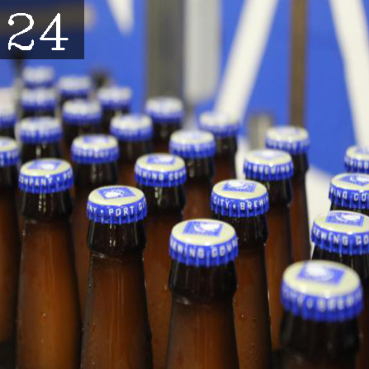
\includegraphics[width=0.16\linewidth]{../files/ABC123/images/fsc_examples/gt/1996_24.png}\hspace{0.1mm}%
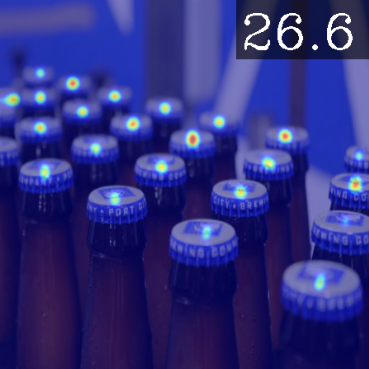
\includegraphics[width=0.16\linewidth]{../files/ABC123/images/fsc_examples/pr/1996_26.6.png}\hspace{0.99mm}%
 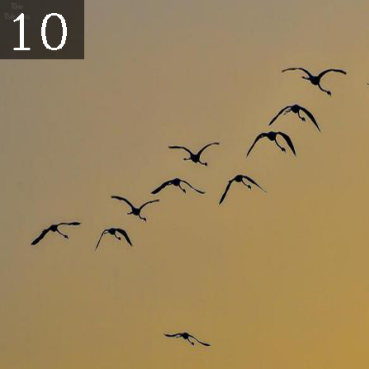
\includegraphics[width=0.16\linewidth]{../files/ABC123/images/fsc_examples/gt/580_10.png}\hspace{0.1mm}%
 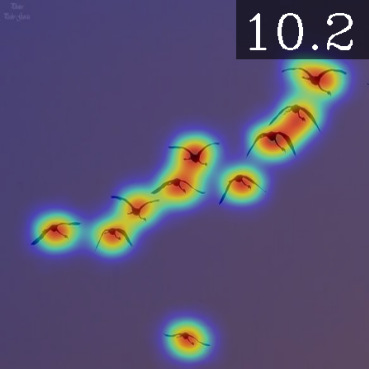
\includegraphics[width=0.16\linewidth]{../files/ABC123/images/fsc_examples/pr/580_10.2.png}\hspace{0.99mm}%
 
\includegraphics[width=0.16\linewidth]{../files/ABC123/images/fsc_examples/gt/1971_19.png}\hspace{0.1mm}%
 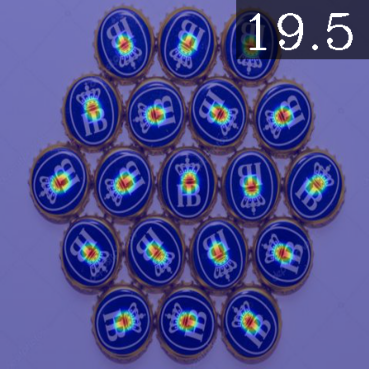
\includegraphics[width=0.16\linewidth]{../files/ABC123/images/fsc_examples/pr/1971_19.5.png}\\ \vspace{0.45mm}
 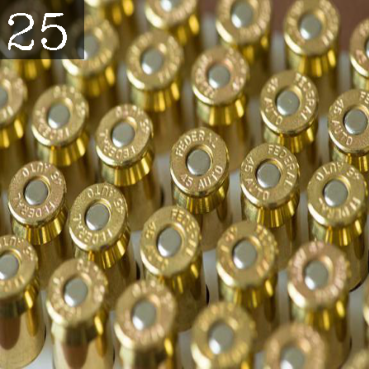
\includegraphics[width=0.16\linewidth]{../files/ABC123/images/fsc_examples/gt/3267_25.png}\hspace{0.1mm}%
 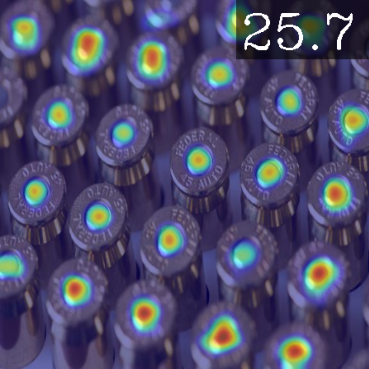
\includegraphics[width=0.16\linewidth]{../files/ABC123/images/fsc_examples/pr/3267_25.7.png}\hspace{0.99mm}%
 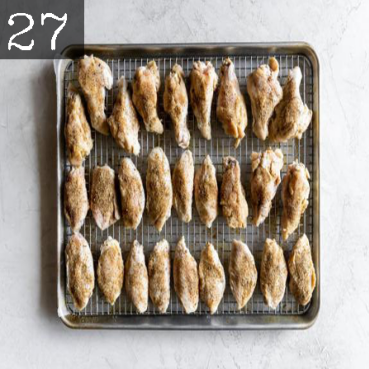
\includegraphics[width=0.16\linewidth]{../files/ABC123/images/fsc_examples/gt/3522_27.png}\hspace{0.1mm}%
 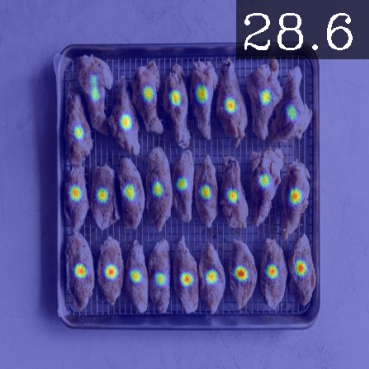
\includegraphics[width=0.16\linewidth]{../files/ABC123/images/fsc_examples/pr/3522_28.6.png}\hspace{0.99mm}%
 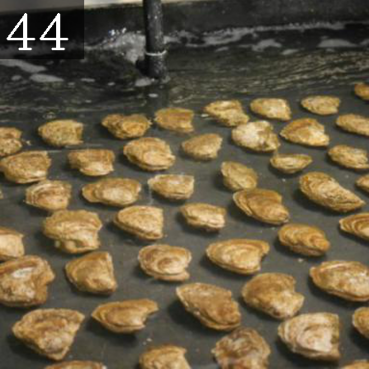
\includegraphics[width=0.16\linewidth]{../files/ABC123/images/fsc_examples/gt/4104_44.png}\hspace{0.1mm}%
 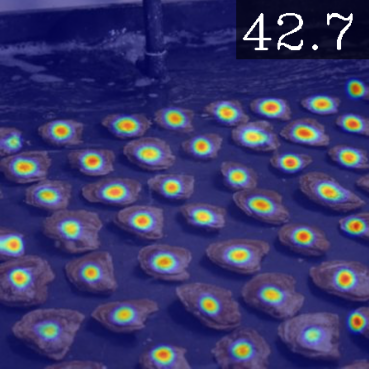
\includegraphics[width=0.16\linewidth]{../files/ABC123/images/fsc_examples/pr/4104_42.7.png}\\ \vspace{0.45mm}
 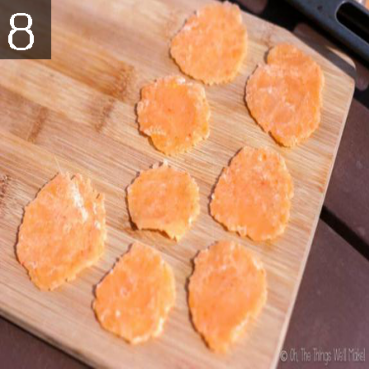
\includegraphics[width=0.16\linewidth]{../files/ABC123/images/fsc_examples/gt/4139_8.png}\hspace{0.1mm}%
 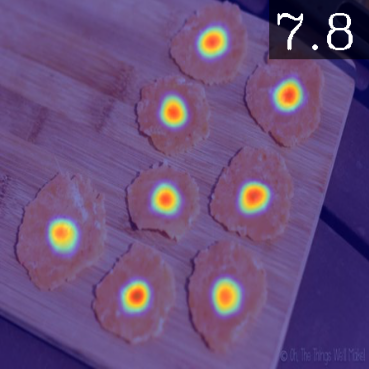
\includegraphics[width=0.16\linewidth]{../files/ABC123/images/fsc_examples/pr/4139_7.8.png}\hspace{0.99mm}%
 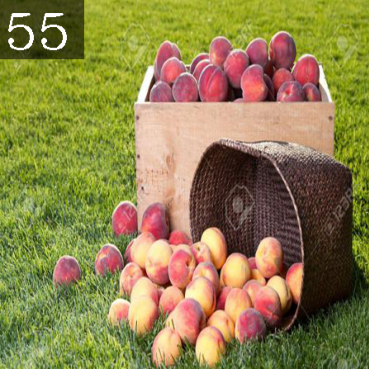
\includegraphics[width=0.16\linewidth]{../files/ABC123/images/fsc_examples/gt/4747_55.png}\hspace{0.1mm}%
 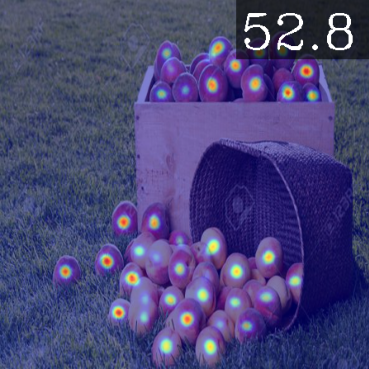
\includegraphics[width=0.16\linewidth]{../files/ABC123/images/fsc_examples/pr/4747_52.8.png}\hspace{0.99mm}%
 
\includegraphics[width=0.16\linewidth]{../files/ABC123/images/fsc_examples/gt/7487_18.png}\hspace{0.1mm}%
 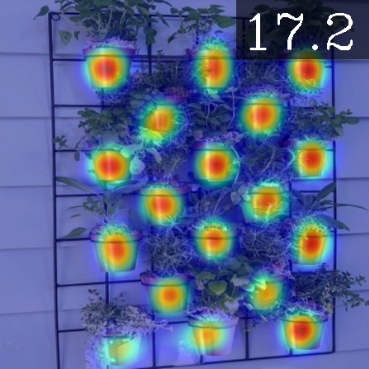
\includegraphics[width=0.16\linewidth]{../files/ABC123/images/fsc_examples/pr/7487_17.2.png}\\ \vspace{0.45mm}
 
\includegraphics[width=0.16\linewidth]{../files/ABC123/images/fsc_examples/gt/7582_25.png}\hspace{0.1mm}%
 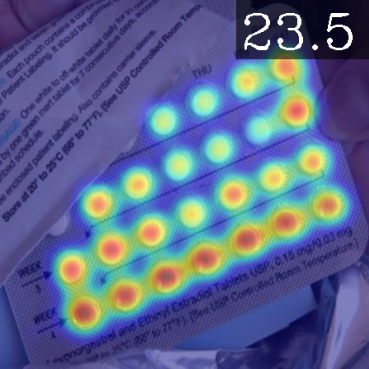
\includegraphics[width=0.16\linewidth]{../files/ABC123/images/fsc_examples/pr/7582_23.5.png}\hspace{0.99mm}%
 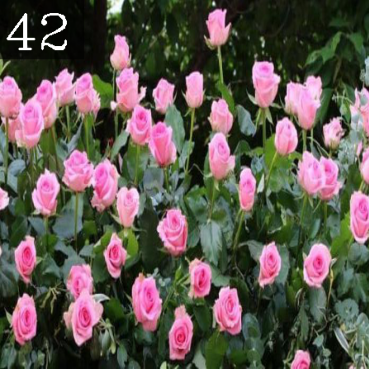
\includegraphics[width=0.16\linewidth]{../files/ABC123/images/fsc_examples/gt/7265_42.png}\hspace{0.1mm}%
 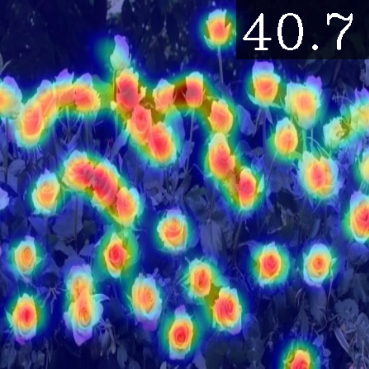
\includegraphics[width=0.16\linewidth]{../files/ABC123/images/fsc_examples/pr/7265_40.7.png}\hspace{0.99mm}%
 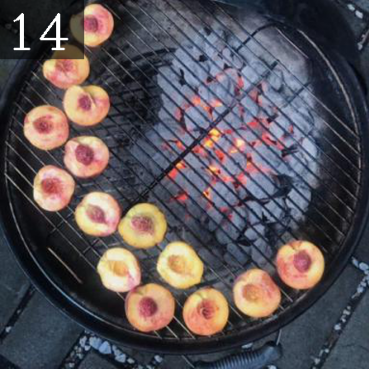
\includegraphics[width=0.16\linewidth]{../files/ABC123/images/fsc_examples/gt/4756_14.png}\hspace{0.1mm}%
 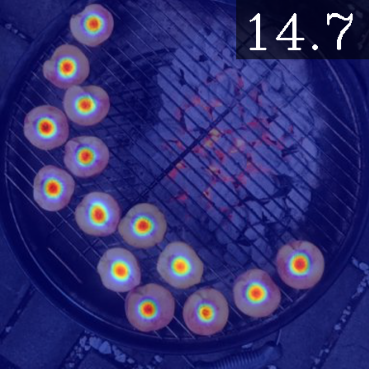
\includegraphics[width=0.16\linewidth]{../files/ABC123/images/fsc_examples/pr/4756_14.7.png}\\ \vspace{0.45mm}
 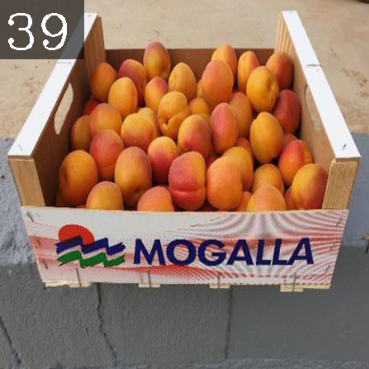
\includegraphics[width=0.16\linewidth]{../files/ABC123/images/fsc_examples/gt/4746_39.png}\hspace{0.1mm}%
 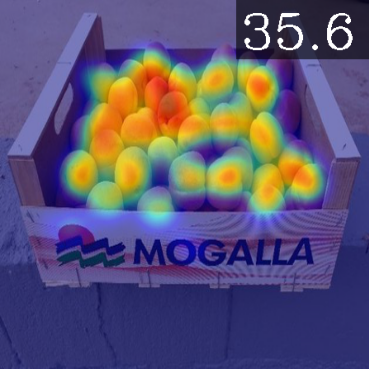
\includegraphics[width=0.16\linewidth]{../files/ABC123/images/fsc_examples/pr/4746_35.6.png}\hspace{0.99mm}%
 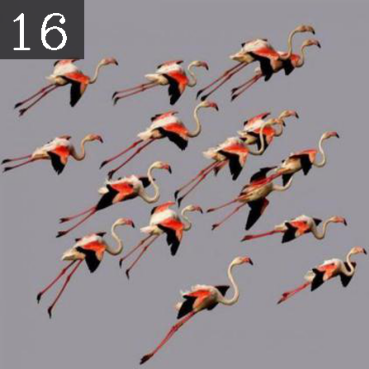
\includegraphics[width=0.16\linewidth]{../files/ABC123/images/fsc_examples/gt/4539_16.png}\hspace{0.1mm}%
 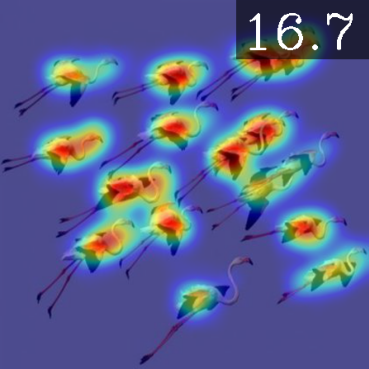
\includegraphics[width=0.16\linewidth]{../files/ABC123/images/fsc_examples/pr/4539_16.7.png}\hspace{0.99mm}%
 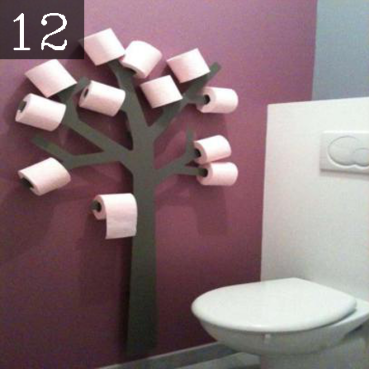
\includegraphics[width=0.16\linewidth]{../files/ABC123/images/fsc_examples/gt/3672_12.png}\hspace{0.1mm}%
 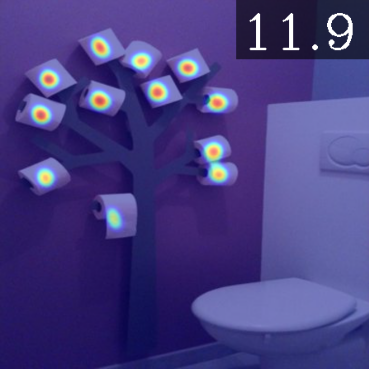
\includegraphics[width=0.16\linewidth]{../files/ABC123/images/fsc_examples/pr/3672_11.9.png}\\ \vspace{0.45mm}
 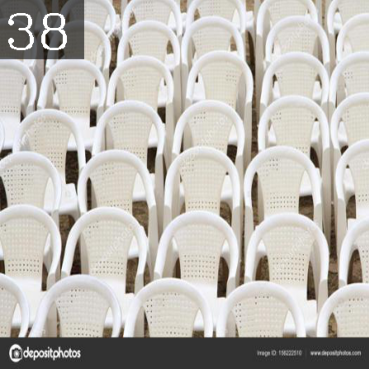
\includegraphics[width=0.16\linewidth]{../files/ABC123/images/fsc_examples/gt/2860_38.png}\hspace{0.1mm}%
 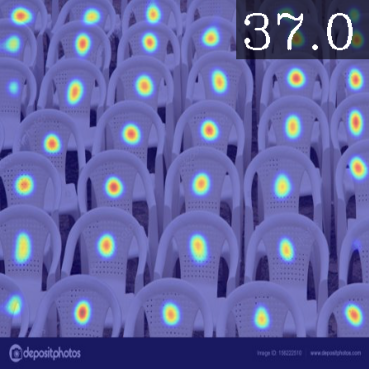
\includegraphics[width=0.16\linewidth]{../files/ABC123/images/fsc_examples/pr/2860_37.0.png}\hspace{0.99mm}%
 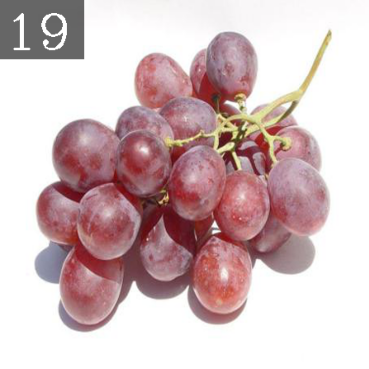
\includegraphics[width=0.16\linewidth]{../files/ABC123/images/fsc_examples/gt/4814_19.png}\hspace{0.1mm}%
 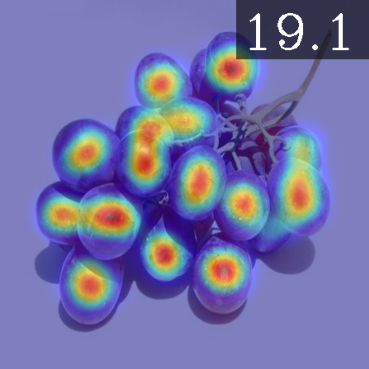
\includegraphics[width=0.16\linewidth]{../files/ABC123/images/fsc_examples/pr/4814_19.1.png}\hspace{0.99mm}%
 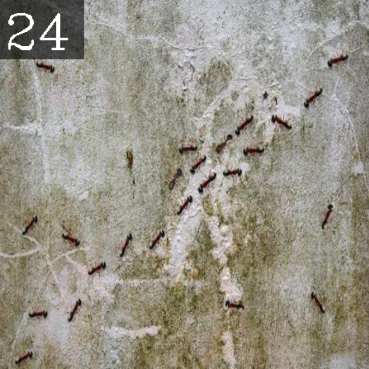
\includegraphics[width=0.16\linewidth]{../files/ABC123/images/fsc_examples/gt/7568_24.png}\hspace{0.1mm}%
 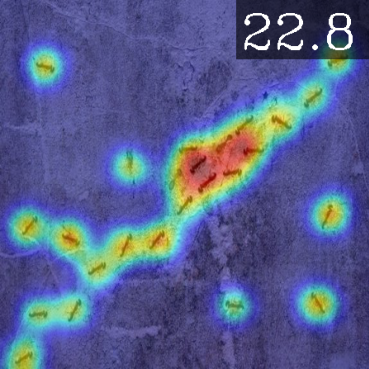
\includegraphics[width=0.16\linewidth]{../files/ABC123/images/fsc_examples/pr/7568_22.8.png}\\ \vspace{0.45mm}%
 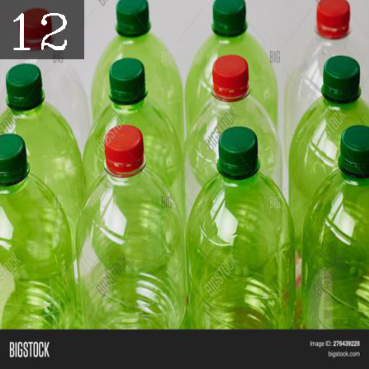
\includegraphics[width=0.16\linewidth]{../files/ABC123/images/fsc_examples/gt/1958_12.png}\hspace{0.1mm}%
 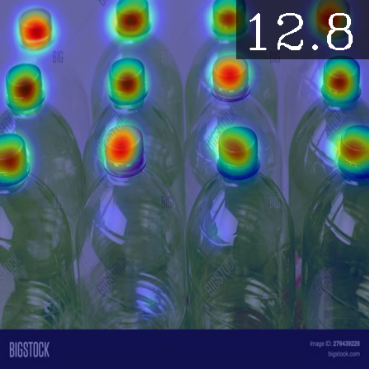
\includegraphics[width=0.16\linewidth]{../files/ABC123/images/fsc_examples/pr/1958_12.8.png}\hspace{0.99mm}%
 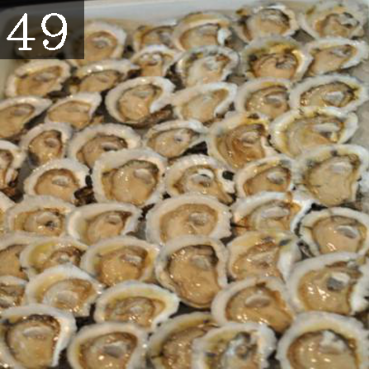
\includegraphics[width=0.16\linewidth]{../files/ABC123/images/fsc_examples/gt/4108_49.png}\hspace{0.1mm}%
 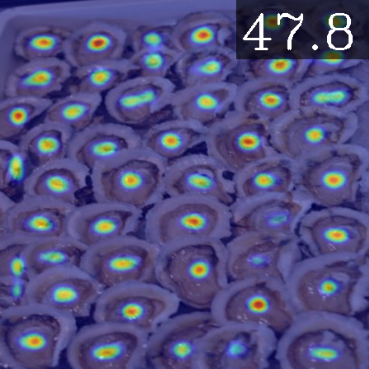
\includegraphics[width=0.16\linewidth]{../files/ABC123/images/fsc_examples/pr/4108_47.8.png}\hspace{0.99mm}%
 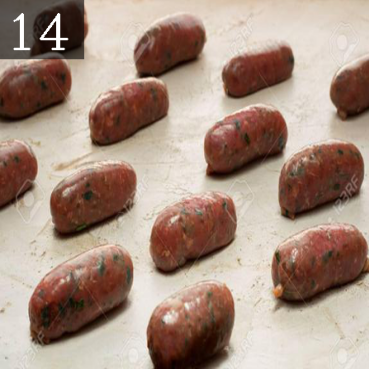
\includegraphics[width=0.16\linewidth]{../files/ABC123/images/fsc_examples/gt/4164_14.png}\hspace{0.1mm}%
 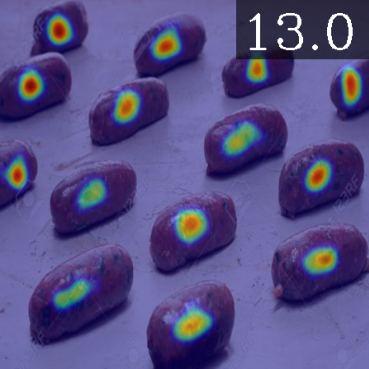
\includegraphics[width=0.16\linewidth]{../files/ABC123/images/fsc_examples/pr/4164_13.0.png}%

        \caption{
    \textbf{ABC123 trained on MCAC generates accurate counts on unambiguous images from FSC}. 
    The input image and ground truth count (top left) and the regressed density map with the predicted count (top right) are shown.
    }
    \label{fig__ABC123__blender_fsc_examples_easy}
\end{figure}


\begin{figure}
    \centering
    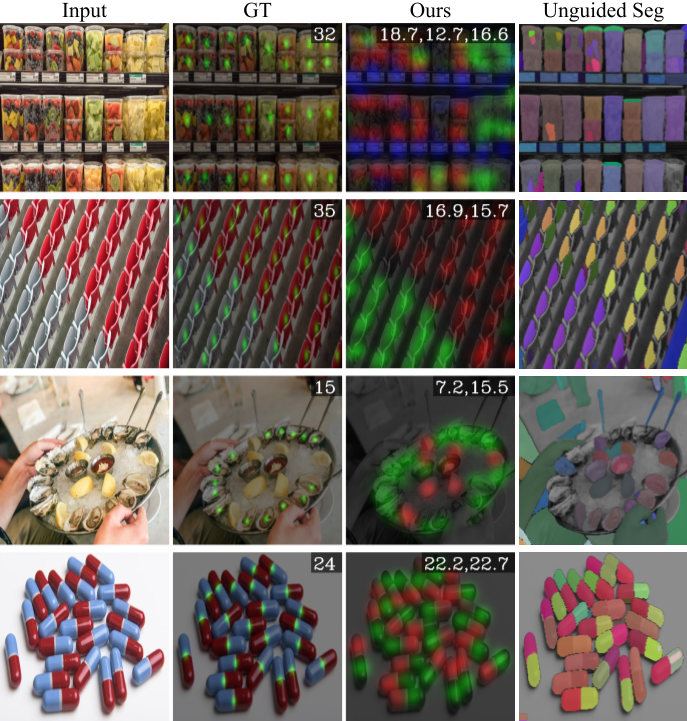
\includegraphics[width=\linewidth]{../files/ABC123/images/added_SAM_outputs.png}
        \caption{
    \textbf{ABC123 trained on MCAC applied to ambiguous images from FSC-133}.    
    ABC123 generates accurate counts for the classes it locates. However, these classes are often not aligned with the human annotations. ABC123 often discovers unlabelled classes, divides labelled classes into sub-classes by colour or shape, or counts the same object multiple times by subdividing each object into component parts.
    Column 2: the ground truth (GT) density map is overlaid in green, Column 3: the predicted density maps are overlaid in red, green, and blue, with the associated counts in the the top corner, Column 4: The outputs of an unguided segmentation method, coloured by feature similarity.
    }
    \label{fig__ABC123__blender_fsc_examples_ambiguos}
\end{figure}


\begin{table}
    \centering
    \resizebox{0.99\textwidth}{!}{%
    \begin{tabular}{lccrrrrrrrr}
 \toprule

 & & \multirow{2}{*}{\shortstack{\vspace{0.6mm}\\Sub-Class \hspace{1mm}\\ Combine}} & \multicolumn{4}{c}{Val Set} & \multicolumn{4}{c}{Test Set} \\
 \cmidrule(r){4-7} \cmidrule(r){8-11}

\multicolumn{1}{c}{Method} & \multicolumn{1}{c}{Shots} &  & \multicolumn{1}{c}{MAE} & \multicolumn{1}{c}{RMSE} & \multicolumn{1}{c}{NAE} & \multicolumn{1}{c}{SRE} & \multicolumn{1}{c}{MAE} & \multicolumn{1}{c}{RMSE} & \multicolumn{1}{c}{NAE} & \multicolumn{1}{c}{SRE} \\

\midrule

\multicolumn{5}{l}{\textit{Exemplar-based}}\\ 

FamNet+ & 3 & N/A & 25.83 & 46.31  & 0.50 & 4.29 & 28.05 & 45.59  & 0.48 & 4.33 \\
BMNet+ & 3 & N/A  & 29.47 & 53.15  & 0.51 & 4.72 & 30.74 & 52.00  & 0.47 & 4.68 \\
CounTR  & 3 & N/A  & 21.22 & 40.28  & 0.47 & 3.85 & 21.09 & 40.79  & 0.38 & 3.66 \\
LOCA  & 3 & N/A &  25.70  & 48.64  & 0.45  & 4.30 & 29.93  & 49.89  & 0.48  & 4.62

\\


\midrule
\multicolumn{5}{l}{\textit{Exemplar-free}} \\
CounTR \dag  & 0 & N/A & 23.50 & 45.83 & 0.42 & 4.06 & 23.57 & 42.00 & 0.39 & 3.85 \\
LOCA  & 0 & N/A & 29.37  & 54.01  & 0.51  & 4.84 & 33.96  & 56.66  & 0.53  & 5.17\\
ABC123  & 0 & Max & \textit{19.56} & 46.71 & \textit{0.20} & \textit{3.54} & \textit{22.43} & 47.35 & \textit{0.22} & \textit{3.70}\\
ABC123  & 0 & Sum & \textbf{11.13} & \textbf{34.47} & \textbf{0.12} & \textbf{2.44} & \textbf{11.75} & \textbf{33.41} & \textbf{0.11} & \textbf{2.38}\\

\bottomrule
\end{tabular}

}
    \caption{Comparison to SOTA methods when trained on MCAC and applied to the cases in FSC147 with fewer than 300 objects. 
     Combining sub-class density maps with a sum rather than a max is more effective as it is more accurate in cases where instances of the sub classes are spatially close or overlapping as both instances are counted completely.
    CounTR \dag \enspace is an exemplar-free modification of CounTR.
    }
    \label{table__ABC123__FSC147_results_table}
\end{table}

\begin{table}
    \centering
   
    \begin{tabular}{lcccc}
 \toprule
Method&MAE&RMSE&NAE&SRE\\
\midrule
\multicolumn{5}{l}{\textit{Exemplar-based}}\\
FamNet+&60.53&84.00&1.82&14.58\\
FSOD &61.31&64.10&1.02&6.94\\
FSDetView \cite{xiao2022few} &24.89&31.34&0.54&4.46\\
Counting-DETR &18.51&\textbf{24.48}&0.45&3.99\\
\midrule
\multicolumn{5}{l}{\textit{Exemplar-free}} \\
ABC123 & \textbf{16.63} & 35.30 & \textbf{0.17} & \textbf{3.02}\\
\bottomrule
\end{tabular}
    \caption{Comparison to the relevant SOTA methods when trained on MCAC and applied to the test set of FSCD-LVIS \cite{nguyen2022few}. 
     Combining sub-class density maps with a max operation.}
    \label{table__ABC123__FSCLVIS_results_table}
\end{table}

\section{Ablations}
In this section, we explain and validate various design decisions including our loss and matching stage scaling.
We also show the effects of generating large numbers of predictions and penalising valid-but-unknown counts on quantitative benchmarks.

\subsection{Validating Our Loss}\label{sec__ABC123__ablation_losses}
We showed in \Cref{sec__LTCA} that using image-wise count loss functions, like the absolute count error, can be beneficial over pixel-wise loss functions as they allow a network to learn its own idea of positional salience.
To validate our choice of a pixel-wise loss function for this more complex task, we test our loss, the pixel-wise error $||d - \hat{d}||_1$, against both the pixel-wise error squared $||d - \hat{d}||^2_2$, as in \cite{ranjan2021Famnet, liu2022countr, xu2023zsc}, and the image-wise count percentage error $|y - \hat{y}|/y$ where $d$ and $\hat{d}$ are the ground truth and predicted density maps, and  $y$ and $\hat{y}$ are the ground truth and predicted counts.

Using an image-wise count loss creates poor results with somewhat arbitrary density maps and high count errors; see \Cref{table__ABC123__ablation_losses}. 
This is likely due to two factors: an increased level of ambiguity and the matching stage now operating on latent features. 
As the multi-class tasks have significantly more ambiguity than their single-class counterparts, it is more difficult for a network to learn a robust idea of the correct positional salience with only integer labels. 
The significant change over the pixel-wise supervision is that the matcher which usually operates on the density map to which the loss is directly applied now operates over an unconstrained latent feature. This, along with the added complexity of multi-class images, makes the problem significantly more difficult to understand from purely integer supervision. 
Matching to the scalar count while using pixel-wise supervision has similar results to matching to the latent features with the overall accuracy being approximately $7\%$ worse.

Using a pixel-wise L$_2$ loss slightly degrades the performance compared to using the L$_1$ distance between the ground truth and predicted density maps. 
Still, the predicted density maps are qualitatively meaningful. 
This discrepancy is likely due to the increased significance the higher-density edge cases have on the training. See \Cref{table__ABC123__ablation_losses} for the quantitative comparison.




\begin{table}
    \centering
    \resizebox{\textwidth}{!}{%
    
\begin{tabular}{lrrrrrrrrr}
    \toprule
    & & \multicolumn{4}{c}{Val Set} & \multicolumn{4}{c}{Test Set} \\
    \cmidrule(r){3-6} \cmidrule(r){7-10}
   
   \multicolumn{1}{c}{Method} & \multicolumn{1}{c}{Loss} & \multicolumn{1}{c}{MAE} & \multicolumn{1}{c}{RMSE} & \multicolumn{1}{c}{NAE} & \multicolumn{1}{c}{SRE} & \multicolumn{1}{c}{MAE} & \multicolumn{1}{c}{RMSE} & \multicolumn{1}{c}{NAE} & \multicolumn{1}{c}{SRE} \\
   \midrule
   
   ABC123 \textsmaller[2]{\SnowflakeChevron} & Count-MAPE & 19.88 & 38.20 & 0.48 & 3.62 & 25.32 & 49.18 & 0.52 & 4.28 \\  
   ABC123 \textsmaller[2]{\SnowflakeChevron} & Pixel $L_2$ & 16.46 & 26.54 & 0.78 & 4.79 & 17.92 & 28.88 & 0.75 & 4.77 \\
   ABC123 \textsmaller[2]{\SnowflakeChevron} & Pixel $L_1$ & \textbf{14.64} & \textbf{23.67} & \textbf{0.46} & \textbf{2.97} & \textbf{15.76} & \textbf{25.72} & \textbf{0.45} & \textbf{3.11}  \\
   \\

   ABC123   & Count-MAPE &  15.95 & 29.71 & 0.50 & 3.54 & 16.28 & 29.82 & 0.49 & 3.58 \\        
   ABC123  & Pixel $L_2$ & 10.76 & 19.31 & 0.49 & 3.84 & 11.91 & 21.42 & 0.51 & 4.21 \\

   ABC123  & Pixel $L_1$ & \textbf{8.96} & \textbf{15.93} & \textbf{0.29} & \textbf{2.02} & \textbf{9.52} & \textbf{17.64} & \textbf{0.28} & \textbf{2.23}  \\


        
   \bottomrule
   \end{tabular}
   
    }
    \caption{The effect of different loss functions during training. Pixel-wise $L_1$ loss produces significantly better results than the pixel-wise $L_2$ loss and the count-wise MAPE.
    }
    \label{table__ABC123__ablation_losses}
\end{table}


\subsection{Validating Our Matching Scaling}\label{sec__ABC123__ablation_matchers}
Normalising the density maps during training and testing is beneficial. 
We hypothesise that this is because it forces the network to generate the correct localisation early in the training as well as the correct magnitude. 
This normalisation also decreases the significance of the issue of the matcher cheating to find the correct count.
Instead of selecting the correct count from a large set of predicted counts, the network must generate a density map with a relevant localisation.
Using the L$_2$ normalisation over the L$_\infty$ has a slight performance increase for training the network and during evaluation. 
We believe this is due to the decreased importance of very high-density areas in images having an overly strong effect on the training.
See \Cref{table__ABC123__ablation_normalised_matching} for a quantitative comparison of the normalisations during the matching stage.
\begin{table}
    \centering
   \resizebox{\textwidth}{!}{%
   
\begin{tabular}{lccrrrrrrrr}
    \toprule
    & \multicolumn{2}{c}{Normalisation}& \multicolumn{4}{c}{Val Set} & \multicolumn{4}{c}{Test Set} \\
    \cmidrule(r){2-3} \cmidrule(r){4-7} \cmidrule(r){8-11}
   
   \multicolumn{1}{c}{Method} & \multicolumn{1}{c}{Train} &  \multicolumn{1}{c}{Eval} & \multicolumn{1}{c}{MAE} & \multicolumn{1}{c}{RMSE} & \multicolumn{1}{c}{NAE} & \multicolumn{1}{c}{SRE} & \multicolumn{1}{c}{MAE} & \multicolumn{1}{c}{RMSE} & \multicolumn{1}{c}{NAE} & \multicolumn{1}{c}{SRE} \\
   \midrule
   
ABC123  \textsmaller[2]{\SnowflakeChevron} & None  & None & 20.31 & 32.40 & 0.78 &  5.40 &  22.67 & 36.63 & 0.92 & 7.25 \\
ABC123  \textsmaller[2]{\SnowflakeChevron} & None  & L$_2$ & 
21.38 & 35.08 & 0.86 & 6.43 & 25.46 & 43.37 & 1.05 & 8.67 \\
ABC123  \textsmaller[2]{\SnowflakeChevron} & None  & L$_\infty$ & 20.13 & 32.15 & 0.81 & 5.86 & 22.76 & 36.78 & 0.95 & 7.64
\vspace{1.5mm}\\
ABC123  \textsmaller[2]{\SnowflakeChevron} & L$_2$ & None & 41.20 & 66.04 & 0.87 & 6.22 & 45.04  & 73.41 & 0.87 & 6.51\\
ABC123  \textsmaller[2]{\SnowflakeChevron} & L$_2$ & L$_2$ & \textbf{14.64} & \textbf{23.67} & \textbf{0.46} & \textbf{2.97} & \textbf{15.76} & \textbf{25.72} & \textbf{0.45} & \textbf{3.11} \\
ABC123  \textsmaller[2]{\SnowflakeChevron} & L$_2$  & L$_\infty$ & 
 17.21 & 27.94 & 0.51 & 3.28 & 17.97 & 29.36 & 0.48 & 3.30\vspace{1.5mm}\\
ABC123  \textsmaller[2]{\SnowflakeChevron} & L$_\infty$  & None & 22.40 & 35.80 & 0.73 & 4.89 & 23.93 & 38.59 & 0.80 & 5.86\\
ABC123  \textsmaller[2]{\SnowflakeChevron} & L$_\infty$  & L$_2$ & 17.92 & 28.98 & 0.67 & 5.12 & 20.40 & 33.39 & 0.77 & 6.24\\
ABC123  \textsmaller[2]{\SnowflakeChevron} & L$_\infty$  & L$_\infty$ & 19.33 & 30.75 & 0.67 & 4.77 & 20.84 & 33.61 & 0.74 & 5.91 \vspace{1.5mm}\\
ABC123   & None  & None & 15.46 & 28.49 & 0.60 & 5.12 &  16.15 & 29.82 & 0.69 & 6.50\\
ABC123   & None  & L$_2$ & 14.83 & 27.25 & 0.68 & 6.15 & 17.04 & 31.88 & 0.84 & 8.06\\
ABC123   & None  & L$_\infty$ & 14.75 & 27.41 & 0.65 & 5.92 & 16.54 & 30.80 & 0.77 & 7.45\vspace{1.5mm}\\
ABC123  & L$_2$ & None & 35.29 & 61.12 & 0.67 & 5.55 & 38.15 & 67.89 &  0.64 &  5.78 \\
ABC123  & L$_2$ & L$_2$ & \textbf{8.96} & \textbf{15.93} & \textbf{0.29} & \textbf{2.02} & \textbf{9.52} & \textbf{17.64} & \textbf{0.28} & 2.23\\
ABC123  & L$_2$ & L$_\infty$ & 9.95 & 18.16 & 0.32 & 2.22 & 9.89 & 18.55 & 0.29 & \textbf{2.20}\vspace{1.5mm}\\
ABC123  & L$_\infty$ & None & 15.72 & 28.83 & 0.59 & 4.69 & 16.11 & 30.22 & 0.67 & 6.16\\
ABC123   & L$_\infty$  & L$_2$ & 12.17 & 22.81 & 0.57 & 5.09 & 13.97 & 27.66 & 0.71 & 7.05 \\
ABC123   & L$_\infty$  & L$_\infty$ & 12.46 & 23.00 & 0.56 & 4.90 & 13.96 & 27.12 & 0.66 & 6.37\\

   
   \bottomrule
   \end{tabular}
   
   }
    \caption{Effect of using normalised density maps for the matching stage. Normalisation improves the accuracy of ABC123. $L_2$ normalisation is more effective than $L_\infty$ during training and evaluation.
    }
    \label{table__ABC123__ablation_normalised_matching}
\end{table}

\subsection{Validating Our Number of Predictions}\label{sec__ABC123__ablation_mhat}

As hypothesised, generating much larger numbers of predictions ($\hat{m} > 5$) increases the quantitative performance of the network; see \Cref{table__ABC123__ablation_mhat} for the complete results. In these cases, the network generates a more diverse set of counts and uses the matching stage to select the best one. 
We believe, however, that this increased quantitative performance does not align with a more useful network in most real-world deployment situations. 
The numerical gain derives purely from the matching stage, which is not present during deployment. 
In fact, during deployment, these configurations would correspond to outputs which are much more difficult to interpret as a user would have to figure out which of the many outputs was most relevant to their problem.

While increasing the number of heads increases the options that can be generated, the return on useful heads diminishes.
When high numbers of heads are used, fewer than half of the generated counts are used, \ie the outputs of some heads were never picked by the matcher. 
See \Cref{table__ABC123__ablation_mhat} for the head utilisation data. 
This is likely due to these heads not being matched frequently during training, meaning a loss is rarely propagated back through them. 

There is also significant redundancy between the heads. The predictions of certain heads over the whole dataset are clearly similar and can be grouped. 
During our testing, of the 39 utilised heads, there were three groups of, respectively, 13, 6, and 4 heads that were very similar, lowering the effective number of utilised heads to 19. 

\begin{table}
    \centering
    \resizebox{\textwidth}{!}{%
    \begin{tabular}{cccccccccccc} 
 \toprule
 & \multicolumn{4}{c}{Val Set} & \multicolumn{4}{c}{Test Set} & \\
 \cmidrule(r){2-5} \cmidrule(r){6-9}

$\hat{m}$ & \multicolumn{1}{c}{MAE} & \multicolumn{1}{c}{RMSE} & \multicolumn{1}{c}{NAE} & \multicolumn{1}{c}{SRE} & \multicolumn{1}{c}{MAE} & \multicolumn{1}{c}{RMSE} & \multicolumn{1}{c}{NAE} & \multicolumn{1}{c}{SRE} & Head Utilisation\\ 
\midrule
4 & 9.43 & 17.42 & 0.32 & 2.57 &10.19 & 19.44 & 0.33 & 2.81 & 100\% \\ 
5 & 8.96 & 15.93 & 0.29 & 2.02 & 9.52 & 17.64 & 0.28 & 2.23 & 100\% \\ 
10 & 8.39 & 14.93 & 0.28 & 1.97 & 9.08 & 16.96 & 0.27 & 2.15 & 100\%\\ 
20 & 7.78 & 13.75 & 0.26 & 1.82 & 8.29 & 15.53 & 0.24 & 1.95 & 85\%\\ 
50 & 7.26 & 12.80 & 0.25 & 1.69 & 7.99 & 15.14 & 0.24 & 1.81 & 68\%\\ 
100 & 7.11 & 12.81 & 0.23 & 1.59 & 7.43 & 14.48 & 0.21 & 1.72 & 39\%\\ 
 \bottomrule
\end{tabular}
 







 
 
 
    }
    \caption{Effect of using more count regression heads. Increasing the number of pre-matching predictions improves the quantitative results of our method. However, as the number of heads increases, the percentage of heads that are frequently ($>0.4\%$) matched decreases.}
    \label{table__ABC123__ablation_mhat}
\end{table}



\begin{figure}
    \centering  
    \begin{subfigure}{0.49\linewidth}
        \centering
                \input{files/ABC123/figures/mhat_results}
    \end{subfigure}
        \begin{subfigure}{0.49\linewidth}
        \centering
                \input{files/ABC123/figures/mhat_utilisation}
    \end{subfigure}
    \caption{Effect of using more count regression heads on the accuracy of ABC123 and the head utilisation.}
    \label{fig__ABC123__ablation_mhat}
\end{figure}



\subsection{Validating Valid-But-Unknown Predictions}\label{sec__ABC123__ablation_vbu}
Here, we show the importance of allowing the generation of valid-but-unknown counts to the success of exemplar-free multi-class class-agnostic counting methods.
To test the effect of allowing the network to generate predictions for unlabelled classes uninhibited, we evaluate the performance of ABC123 when the loss is applied to all $\hat{m}$ predictions and as before applying it to only the $m$ matched predictions.
When the method is encouraged to generate blank density maps and zero counts for everything but the labelled counts the accuracy is significantly worse.
The network generates counts and density maps which are consistently too low. 
Not only does forcing the network to generate zeros for unlabelled counts harm the networks ability to gain its own nuanced understanding of counting, it also lowers the signal-to-noise ratio of meaningful counting information during training. 
As most of the images present in MCAC have less than half of the maximum number of types of objects, see \Cref{fig__multi_class_stats_graphs}, the network is motivated to generate 0 most of the time during training.
The results are presented in \Cref{table__ABC123__ablation_VBU}.

This shows the clear advantage of allowing the network to generate counts associated with divisions that were not specified by the dataset labels.
This is because the network is able to generate more nuanced representations of counting when it is not encumbered with arbitrary rules of what is a `valid' count.
It should be noted that even with the stricter loss, ABC123 is still superior to contemporary methods. 

\begin{table}
    \centering
    \begin{tabular}{cccccccccccc} 
 \toprule
 & & \multicolumn{4}{c}{Val Set} & \multicolumn{4}{c}{Test Set} & \\
 \cmidrule(r){3-6} \cmidrule(r){7-10}
$\hat{m}$ & loss applied to &\multicolumn{1}{c}{MAE} & \multicolumn{1}{c}{RMSE} & \multicolumn{1}{c}{NAE} & \multicolumn{1}{c}{SRE} & \multicolumn{1}{c}{MAE} & \multicolumn{1}{c}{RMSE} & \multicolumn{1}{c}{NAE} & \multicolumn{1}{c}{SRE} \\ 
\midrule
4 & all & 33.66 & 49.15 & 0.87 & 6.83 & 36.41 & 54.88 & 0.91 & 7.14 \\
4 & $m$ & 9.43 & 17.42 & 0.32 & 2.57 & 10.19 & 19.44 & 0.33 & 2.81 \\
5 & all & 23.08 & 42.66 & 0.84 & 5.35 & 24.99 & 47.87 & 0.75 & 5.64 \\
5 & $m$ & 8.96 & 15.93 & 0.29 & 2.02 & 9.52 & 17.64 & 0.28 & 2.23 \\

 \bottomrule
\end{tabular}
    \caption{Effect of applying the loss to all regressed counts compared to only the matched counts. When the loss is only applied to the matched $m$ predictions, it is able to generate counts associated with unlabelled divisions. When the loss is applied to all $\hat{m}$ predictions, all of the counts not associated with a count are forced to 0.
    This strict approach damages the training of ABC123 as it reduces the capacity of the network to generate nuanced representations of counting.}
    \label{table__ABC123__ablation_VBU}
\end{table}


\section{Conclusion}
\label{conclusion}
In this chapter, we present ABC123, a multi-class exemplar-free class-agnostic counter, and show that it is superior to prior exemplar-based methods in multi-class settings.
We also show that the understanding of counting ABC123 gains from being trained on synthetic data can be applied to photographic images.
ABC123 requires no human input at inference-time, works in complex settings with more than one kind of object present, and outputs easy-to-understand information in the form of examples of the counted objects.
Due to this, it has good potential for deployment in various fields.

\end{document}